\documentclass{sig-alternate}


\usepackage{enumitem}
\usepackage{framed}
\usepackage{cprotect}
\usepackage{enumitem}
\usepackage{listings}
\usepackage{amstext}
\usepackage{amstext}
\usepackage{pdfpages}
\usepackage{alltt}
\usepackage{epstopdf}
\usepackage{xspace,colortbl}
\usepackage[USenglish]{babel}
\usepackage{multirow}
\usepackage{url}
\usepackage{subfigure}
\usepackage{graphicx}%%
\usepackage{amssymb}
\usepackage{fmtcount}
\usepackage{amsfonts}
\usepackage{xspace}
\usepackage{amsmath}
\usepackage{multirow}
\usepackage[mathscr]{eucal}
%\usepackage{psfrag}
\usepackage{colortbl}

\usepackage{bm}
\usepackage{times}
%\usepackage[nospace]{cite}
\usepackage{csquotes}
\usepackage{enumitem}

\lstset{basicstyle=\large,breaklines=true,language=SQL,belowcaptionskip=.1\baselineskip}

%\linespread{0.975}

\makeatletter
\def\@copyrightspace{\relax}
\makeatother

\begin{document}

%\setlength{\belowdisplayskip}{1pt} \setlength{\belowdisplayshortskip}{1pt}
%\setlength{\abovedisplayskip}{1pt} \setlength{\abovedisplayshortskip}{1pt}
%\setlength{\belowcaptionskip}{-10pt}
%\selectfont

\newtheorem{theorem}{Theorem}
\newtheorem{example}{Example}
\newtheorem{definition}{Definition}
\newtheorem{problem}{Problem}
\newtheorem{property}{Property}
\newtheorem{proposition}{Proposition}
\newtheorem{lemma}{Lemma}
\newtheorem{corollary}{Corollary}

\newcommand{\cond}{\textrm{pred}\xspace}
\newcommand{\dataset}{data set\xspace}
\newcommand{\datasets}{data sets\xspace}
\newcommand{\spview}{\textsf{SPView}\xspace}
\newcommand{\fjview}{\textsf{FJView}\xspace}
\newcommand{\aggview}{\textsf{AggView}\xspace}
\newcommand{\hashfunc}[1]{\textsf{hash}(#1)\xspace}
\newcommand{\hashop}{\textsf{hash}\xspace}
\newcommand{\nsc}{\textsf{NormalizedSC}\xspace}
\newcommand{\rsc}{\textsf{RawSC}\xspace}

\newcommand{\avgfunc}{\ensuremath{\texttt{avg} }\xspace}
\newcommand{\maxfunc}{\ensuremath{\texttt{max} }\xspace}
\newcommand{\minfunc}{\ensuremath{\texttt{min} }\xspace}
\newcommand{\histfunc}{\ensuremath{\texttt{histogram\_numeric} }\xspace}
\newcommand{\countfunc}{\ensuremath{\texttt{count}}\xspace}
\newcommand{\sumfunc}{\ensuremath{\texttt{sum} }\xspace}
\newcommand{\varfunc}{\ensuremath{\texttt{var} }\xspace}
\newcommand{\stdfunc}{\ensuremath{\texttt{std} }\xspace}
\newcommand{\covfunc}{\ensuremath{\texttt{cov} }\xspace}
\newcommand{\corrfunc}{\ensuremath{\texttt{corr} }\xspace}
\newcommand{\medfunc}{\ensuremath{\texttt{median} }\xspace}
\newcommand{\percfunc}{\ensuremath{\texttt{percentile} }\xspace}
\newcommand{\havingfunc}{\ensuremath{\texttt{HAVING} }\xspace}
\newcommand{\selectfunc}{\ensuremath{\texttt{select} }\xspace}
\newcommand{\ratio}{\ensuremath{\rho }\xspace}


\newcommand{\insertion}{\ensuremath{\texttt{INSERT} }\xspace}
\newcommand{\update}{\ensuremath{\texttt{UPDATE} }\xspace}
\newcommand{\delete}{\ensuremath{\texttt{DELETE} }\xspace}

\newcommand{\sysfull}{ActiveClean\xspace}
\newcommand{\sys}{ActiveClean\xspace}
\newcommand{\sysnospace}{ActiveClean}

\newcommand{\tbl}[1]{\textsf{#1}\xspace}
\newcommand{\field}[1]{\textsf{#1}\xspace}
\newcommand{\cost}{\textrm{cost}\xspace}
\newcommand{\ans}{\textsf{ans}\xspace}
\newcommand{\dans}{\Delta\textsf{ans}\xspace}
\newcommand{\cqp}{correction query processing\xspace}
\newcommand{\Cqp}{Correction query processing\xspace}

\newcommand{\reminder}[1]{{{\textcolor{magenta}{\{\{\bf #1\}\}}}\xspace}}
\newcommand{\specialcell}[2][c]{%
  \begin{tabular}[#1]{@{}c@{}}#2\end{tabular}}

\def\ojoin{\setbox0=\hbox{$\bowtie$}%
  \rule[-.02ex]{.25em}{.4pt}\llap{\rule[\ht0]{.25em}{.4pt}}}
\def\leftouterjoin{\mathbin{\ojoin\mkern-5.8mu\bowtie}}
\def\rightouterjoin{\mathbin{\bowtie\mkern-5.8mu\ojoin}}
\def\fullouterjoin{\mathbin{\ojoin\mkern-5.8mu\bowtie\mkern-5.8mu\ojoin}}

%\setlength{\belowcaptionskip}{-10pt}

%\newcommand{\reminder}[1] {}
\pagestyle{plain}

\title{ActiveClean: Progressive Data Cleaning For Convex Data Analytics}

%\numberofauthors{1}
%\author{\large Sanjay Krishnan, Jiannan Wang, Michael J. Franklin, Ken Goldberg, Tim Kraska{$\,^\dag$} \\
%\vspace{.2em}\affaddr{\large UC Berkeley, ~~ $^\dag$Brown University} \\
%\vspace{.1em}\affaddr{\large \{sanjaykrishnan, jnwang, franklin, goldberg\}@berkeley.edu}\\
%\affaddr{\large tim\_kraska@brown.edu}
%}

%\fontsize{10pt}{11pt}
%\selectfont

{\noindent \normalsize \bf Dear PVLDB Chair and Referees: }

\vspace{.5em}
We thank the reviewers and chair for the very helpful feedback on our paper. We have addressed all of the listed concerns and include references to the revised text in the cover letter. 
To summarize :
\begin{enumerate}
\item We revised our background section (Section \ref{subsec-inc}) to include a detailed running example which is referenced in Examples 1-6 after each major concept.
\item We revised our overview section (Section 3) to formalize our problem setting, assumptions, terminology, and key prerequisite concepts.
\item The sampling section (Section 4) included a detailed discussion about the challenges and new ideas (Section 4.1) and clarified a reviewer request about the definition of ``primary keys".
\item The result estimation section (Section 5) has been revised to include itemized descriptions of all of the algorithms and is self-contained with respect to our prior work.
\item The experiments section (Section 7) has been revised to merge redundant experimental results. We feel that the distributed experiment is a valuable contribution since it evaluates the technique at scale and on a real dataset. However, we noticed that the views in the distributed experiment were group by aggregates and we removed a TPCD evaluation of this same class of views.
Rather than presenting two different experimental results, we use our real dataset to evaluate \svc on group by aggregate views, while also discussing the performance at scale. 
\end{enumerate}
We first will detail our changes in response to the meta reviewer comments and then address the detailed reviewer comments subsequently.

\vspace{2em}
\noindent\textbf{[Meta Reviews]}
\vspace{1em}

\emph{M1. The definitions and discussions, which are currently presented in a very hand-waiving manner, need to be replaced with their formal counterparts. The presentation should be revised, also to avoid the continuous references to the tech report for details. Please see the detailed comments E1 of reviewer 1, and C1,C2, C4, C5, and C6 of reviewer 2 for more details.}
\vspace{.25em}

{\bf Responses:} We have significantly clarified the presentation of the concepts and the algorithms. Section 3.1 (Notations and Definitions) has been expanded to formally present the core preliminaries of our work: Materialized Views, Staleness, Relational Expressions for Maintenance, and Uniform Sampling. Section 3.2 presents an itemized workflow of SVC and formal descriptions of the problems that SVC solves. In our sampling section (Section 4), we replace the informal descriptions with their formal counterparts including Definition 1 (Provenance), Proposition 1 (Primary Key based Provenance), and Property 1 (Correspondence). We summarize the intuitions in these formal concepts with Example 3 and Example 4. We revised Section 5 to have an itemized description of the estimation algorithms proposed in this work.  Additionally, the technical report is now only cited in the Experiments section with reference to details in the experimental setup and materialized view choice.

\vspace{1em}
\emph{M2. There are several assumptions and restrictions that are not spelled out clearly in the first part of the paper. It should be clarified how much they limit the applicability of the proposal. The real-world scenarios used is very interesting, but do the techniques apply in other popular applications, where the assumption in sec 4.2 may not hold?}

\vspace{.25em}

{\bf Responses:} We have revised the presentation of the work to be more explicit about limitations. We added the following paragraph before the problem statements in Section 3.1:
\begin{displayquote}In SVC, we explore the problem of approximate aggregate query
processing on stale materialized views using a data-cleaning approach.
We assume that these materialized views are periodically
maintained and thus are stale in between maintenance periods. The
focus of this paper is analytic workloads where the typical query on the view is a group by aggregate. SVC provides a framework for increased
query accuracy for a flexible maintenance cost that can
scale with system constraints.\end{displayquote}

We believe this concisely summarizes our problem domain and applicability of our proposal. 
Furthermore, we have clarified that the primary key definition proposed in 4.2 
(Section 4.3 in the revised paper) is not an assumption but a generation procedure. For the relational expressions described in the paper (select, project, join, aggregate, union, difference), if there is a unique primary key for the base relations, we can ensure that any derived relation also has a unique primary key by the rules described in Definition 2. If the base relations do not have primary keys, then we can add an extra column to the relation that assigns each row a unique id. We added Example 3 and Figure 2 to describe this process concretely.

\vspace{1em}
\emph{M3. There are recent proposals in data cleaning over materialized views that tackle an orthogonal problem: While the setting is different, work has been done on how to use a different statistical measure (sensitivity analysis) to tackle similar technical problems (sec 5.1.1, sec 6.3). The authors can find related techniques in the recent work on data cleaning over views. It would be useful to have a technical discussion of how the proposed techniques can be applied in this related setting and vice versa (an experimental evaluation is not needed): (1) Wu and Madden. Scorpion: Explaining Away Outliers in Aggregate Queries. PVLDB 2013, (2) Chalamalla et al. Descriptive and prescriptive data cleaning. SIGMOD 2014, (3) Meliou et al. Tracing data errors with view-conditioned causality. SIGMOD 2011}

\vspace{.25em}

{\bf Responses:} Thank you for bringing this to our attention.
\svc builds on the prior work about cleaning materialized views by using ideas like provenance.
However, the materialized view maintenance problem setting (with staleness as the source of dirtiness) adds new challenges that prior work does not address.
We have added a paragraph to our related work (Section 8) contrasting these works from \svc:
\begin{displayquote}
\svc shares ideas, such as provenance, with prior work on cleaning materialized views.
Meliou et al. \cite{DBLP:conf/sigmod/MeliouGNS11} proposed a technique to trace errors in an MV to base data and find responsible erroneous tuples. 
They do not, however, propose a technique to correct the errors as in \svc.
Correcting general errors as in Meliou et al. is a hard constraint satisfaction problem.
However, in \svc, through our formalization of staleness, we have a model of how updates to the base data (modeled as errors) affect MVs, which allows us to both trace errors and clean them.
Wu and Madden \cite{DBLP:journals/pvldb/0002M13} did propose a model to correct ``outliers" in an MV through deletion of records in the base data.
This is a more restricted model of data cleaning than \svc, where the Wu and Madden only consider changes to existing rows in an MV (no insertion or deletion) and does not handle the same generality of relational expressions (e.g., nested aggregates).
Challamalla et al. \cite{DBLP:conf/sigmod/ChalamallaIOP14} proposed an approximate technique for specifying errors as constraints on a materialized view and proposing changes to the base data such that these constraints can be satisfied.
While complementary, one major difference between the three works \cite{DBLP:conf/sigmod/MeliouGNS11, DBLP:journals/pvldb/0002M13, DBLP:conf/sigmod/ChalamallaIOP14} and \svc is that they require an explicit specification of erroneous rows in a materialized view.
Identifying whether a row is erroneous requires materialization and thus specifying the errors is equivalent to full incremental maintenance. 
We use the formalism of a ``maintenance strategy", the relational expression that updates the view, to allow us to sample rows that are not yet materialized.
\svc as complementary to these works in the dirty data setting. 
The sampling technique proposed in Section 4 of our paper could be used to approximate the data cleaning techniques in \cite{DBLP:conf/sigmod/MeliouGNS11, DBLP:journals/pvldb/0002M13, DBLP:conf/sigmod/ChalamallaIOP14} and this is an exciting avenue of future work.\end{displayquote}

\vspace{1em}
\emph{M4. The experiments sections needs to be improved to include comparison with relevant work, more details and explanation. Please look at the detailed comments E2, E4, and E5 of reviewer 1, and B1 and B2 of reviewer 2 for more details. }

\vspace{.25em}

{\bf Responses:} We have addressed all of the details in the reviewer section of the cover letter. To summarize, we cited the algorithm that we used for Incremental View Maintenance which is the change-table algorithm (also called a delta table e.g \cite{DBLP:journals/vldb/KochAKNNLS14}) described in “Maintenance of Materialized Views: Problems, Techniques, and Applications” by Gupta et al. \cite{gupta1995maintenance, gupta2006incremental}. 
We further clarified our contribution for the two compared query processing approaches, SVC+ CORR and SVC+AQP. Both techniques use our Stale View Cleaning technique but have a different result estimation procedure. 

There were also reviewer concerns about the selectivity (for which we added a theoretical analysis) and the update size (for which we clarified the experiment in which those results can be seen).
In addition, two reviewers suggested removing our detailed evaluation on a distributed platform to save space. 
We feel that the distributed experiment is a valuable contribution since it evaluates the technique at scale and on a real dataset. However, we noticed that the views in the distributed experiment were group by aggregates and we removed a TPCD evaluation of this same class of views.
Rather than presenting two different experimental results, we use our real dataset to evaluate \svc on group by aggregate views, while also discussing the performance at scale. 
We, however, save space by excluding details on the experimental setup and performance characterization of Apache Spark.

\vspace{1em}
\emph{M5. The paper's main motivation is that eager IVM cannot keep up with the rate of incoming updates. However, there have been approaches in the literature (most notable DBToaster) suggesting that this issue can be resolved by accelerating IVM. Do you think that there is still a need of SVC? What is the rate of updates over which a system such as DBToaster cannot keep up with the updates?}

\vspace{.25em}

{\bf Responses:} Thank you for bringing this to our attention. In the paper (Section 2.1), we have added the following clarification and motivation of the work:
\begin{displayquote}

There has been significant research on fast MV maintenance algorithms, most recently DBToaster \cite{DBLP:journals/vldb/KochAKNNLS14} which uses SQL query compilation and higher-order maintenance.
However, even with these optimizations, some materialized views are computationally difficult to maintain and will have maintenance costs that can grow with the size of data (e.g, correlated aggregate in a sub-query).
Increasingly large views require distribution and this further increases maintenance costs due to coordination.
Furthermore, in real deployments, it is common to use the same infrastructure to maintain multiple materialized views (along with other analytics tasks) adding further contention to computational resources and reducing overall maintenance throughput. 
When faced with these challenges, it is common to batch updates to amortize maintenance overheads and add flexibility to scheduling.
In such settings, we see an opportunity for approximation through sampling which can give bounded query results in rapidly changing data for a reduced maintenance cost.
Any amount of staleness can lead to erroneous query results where the user has no idea about the magnitude or the scope of query error. 
\svc uses a small sample of up-to-date data to return a bounded approximation, which while still approximate, shows the user how far they are from the true answer.
\svc is complementary to the choice of maintenance algorithm and maintenance setting (e.g mini-batch on the order of seconds/minutes or periodic deferral).
\end{displayquote}

We see integration with DBToaster as an exciting opportunity for future work exploring how sampled maintenance plans can be compiled and how \svc integrates with higher-order view maintenance.

\vspace{1em}
\emph{M6. Typos and other minor issues as listed by E6 of reviewer 1 and C7, C8, C9, C10 and C11 of reviewer 2 should be addressed.}

\vspace{.25em}

{\bf Responses:} We thank the reviewers for their careful read of the paper, and have addressed all of these issues.

\vspace{2em}
\noindent\textbf{[Reviewer 1]}
\vspace{1em}

\emph{B1. There are several assumptions and restrictions that are not spelled out clearly in the first part of the paper. It should be clarified how much they limit the applicability of the proposal. The real-world scenarios used is very interesting, but do the techniques apply in other popular applications, where the assumption in sec 4.2 may not hold?}

\vspace{.25em}

{\bf Responses:} This review is addressed above in Meta Review Section (M2).

\vspace{1em}
\emph{B2. It is great to see many technical and engineering contributions, but the paper is very dense and hard to read. The first clear example of what is going on appears at page 4, after the reader had tried hard to understand the problem statement in sec 3.3.1. The presentation should be revised, also to avoid the continuous references to the tech report for details.}

\vspace{.25em}

{\bf Responses:} We have revised the presentation of the work to be easier to follow. In Section 2.1, we describe a running example of Video Streaming Log Analysis. In Section 3, there are two detailed examples of the concepts presented. Example 1 describes the terminology and prerequisite concepts in terms of a concrete use case, and Example 2 illustrates the end-to-end workflow of \svc. In Section 4, we add Example 3 to clarify the reviewer concern about the applicability of primary key lineage in this setting and Example 4 to show how we can optimize sampling of a materialized view in a real application. In Section 5, we add Example 5 to describe our query processing approaches. In Section 6, we add Example 6 to describe how outlier indexing would be used in practice. 

We have further minimized the references to the technical report. The technical report is now only for details in the experimental setup. The theoretical presentation of this work is now self contained with respect to our prior work.

\vspace{1em}
\emph{B3. There are recent proposals in data cleaning over materialized views that tackle an orthogonal problem: given a view, they clean a sample of its data and go back to the base relations to identify useful explanations. While the setting is different, work has been done on how to use a different statistical measure (sensitivity analysis) to tackle similar technical problems (sec 5.1.1, sec 6.3). Given the data cleaning angle of the proposal, a comparison with these techniques is relevant in this work.}

\vspace{.25em}

{\bf Responses:} We address this issue in the Meta Review Section (M3).

\vspace{1em}
\emph{E1. I would recommend the authors to revise the presentation of the paper to make it more accessible to the readers, for example with more examples and by limiting the tech report for relevant information. While it is great to show great engineering effort, I think it would be beneficial for this work to deliver more clearly what are the key intuitions and novel ideas. For example, I am not sure I understand the need to conduct the experiment on a distributed platform, as it doesn't touch any of the key contributions of the work. Of course, it is hard to add examples, comparisons, and clarifications without removing something, but in this case I'd say this experiment could be moved to the tech report to leave more room to clarify the basic ideas of the paper and make it more self-contained (e.g., the discussion on CLT with the ref to [36]).}

\vspace{.25em}

{\bf Responses:} We now summarize our contributions in the introduction as follows:
\begin{displayquote}
(1) we formalize maintenance of a sample MV as a data cleaning operation on the sample, (2) we propose an optimization technique that materializes the clean sample efficiently while preserving correctness, (3) we derive a query processing approach to answer aggregate queries accurately using the clean sample, (4) we propose an outlier index to reduce sensitivity to skewed datasets, and (5) we evaluate our approach on real and synthetic datasets confirming that indeed sampling can reduce view maintenance time while providing accurate query results. 
\end{displayquote}
To make the presentation more accessible, we have revised the work with the clarifying examples described above (B2), and introduced a itemized summary of all of the components in Section 3.2. We have also revised Section 4 (Stale View Cleaning) of the paper with the following clarifications: introducing problem specific challenges (Section 4.1) and a clarified presentation of Provenance (Section 4.2-3). As the reviewer suggested, we have limited the use of the technical report to experimental engineering details. In our submission, many of the details in Section 5 (Query Result Estimation) were omitted and discussed in the technical report. In addition to the clarifying examples described for review B2, we have made the following revisions to Section 5 to make it more accessible: (1) we present itemized algorithms for our query result estimation approaches, (2) we provide SQL descriptions of confidence interval calculations via the CLT, and (3) we present a simpler taxonomy of different families of aggregate queries and their properties. 
To make space for these additional clarifications, we consolidated our experiments. We believe that our distributed experiment is a valuable contribution as it demonstrates the usefulness of sampling at large scales, however, noticing that in this real experiment all of the views were group by aggregates, we removed our ``data cubing" experiment illustrating the same points with real data.

\vspace{1em}
\emph{E2. I would anticipate a discussion on the context in which the approach works. I would also like to understand why it is hard to go beyond the assumptions with a more general discussion. Right now there are limitations spread over the paper: }

\vspace{.25em}

{\bf Responses:} We address the first part of this question in the Meta Review section (M2). For the second part of the question, we expanded the Limitations section (Section~9) at the end of the paper:
\begin{displayquote}
While our experiments show that \svc works for a variety applications, there are a few limitations which we summarize in this section.
There are three primary limitations for \svc: class of queries and types of materialized views. 
In this work, we primarily focused on aggregate queries and showed that accuracy decreases as the selectivity of the query increases.
Sampled-based methods are fundamentally limited in the way they can support ``point lookup" queries that select a single row.
This is predicted by our theoretical result that accuracy decreases with $\frac{1}{p}$ where $p$ is the fraction of rows that satisfy the predicate.
In terms of more view definitions, \svc does not support views with ordering or ``top-k'' clauses, as our sampling assumes no ordering on the rows of the MV and it is not clear how sampling commutes with general ordering operations.
\end{displayquote}

\emph{E2-1. In 3.3.2 for the sql I was also expecting an experiment to see different quality results depending on the selectivity of the query}

\vspace{.25em}

{\bf Responses:} We included a theoretical analysis of selectivity in Section 5.3.3:
\begin{displayquote}
Let $p$ be the selectivity of the query and $k$ be the sample size; that is, a fraction $p$ records from the relation satisfy the predicate.
For these queries, we can model selectivity as a reduction of effective sample size $k\cdot p$ making the
estimate variance: $O(\frac{1}{k*p})$.
Thus, the confidence interval's size is scaled up by $\frac{1}{\sqrt{p}}$.
Just like there is a tradeoff between accuracy and maintenance cost, for a fixed accuracy, 
there is also a tradeoff between answering more selective queries and maintenance cost.
\end{displayquote}
We believe these results are predictable as for a fixed $p$, $\frac{1}{\sqrt{p}}$ is just a constant scaling on the accuracy results.
In our experiments, we randomly generated queries with a variety of different selectivities described in Section 7.1.1:
\begin{displayquote}
For each of the views, we generated \emph{queries on the views}.
Since the outer queries of our views were group by aggregates, we picked a random attribute $a$ from the group by clause and a random attribute $b$ from aggregation.
We use $a$ to generate a predicate.
For each attribute $a$, the domain is specified in the TPCD standard.
We selected a random subset of this domain, e.g., if the attribute is country then the predicate can be $\text{countryCode} > 50$ and $\text{countryCode} < 100$.
We generated 100 random \sumfunc, \avgfunc, and \countfunc queries for each view.
\end{displayquote}
For example, in Figure 5, the average selectivity was 24.1\%.
If we chose twice as selective queries, the errors would scale by up $\sqrt{2} \approx 1.4$.

\vspace{1em}

\emph{E2-2. In 4.2 for the PK requirement  this seems very strong and not realistic in many applications: what if this assumption does not hold? would AQP also fails?}

\vspace{.25em}

{\bf Responses:} We have clarified that the primary key definition proposed in 4.2 (Section 4.3 in the revised paper) is not an assumption but a generation procedure. For the relational expressions described in the paper (select, project, join, aggregate, union, difference), if there is a unique primary key for the base relations, we can ensure that any derived relation also has a unique primary key by the rules described in Definition 2. If the base relations do not have primary keys, then we can add an extra column to the relation that assigns each row a unique id. We added Example 3 and Figure 2 to describe this process concretely.

\vspace{1em}
\emph{E2-3. In 6.1 for the background knowledge is it realistic to have the user defining all these indexes? can also the traditional incremental solution benefit for a similar optimization? you should clarify if the experiments before 7.2.4 are done with or without the indexing. If they all done without the indexing, it seems that your methods does not really needed this optimization}

\vspace{.25em}

{\bf Responses:} We have added clarification on how these indices may be constructed in Section 6.1:
\begin{displayquote}There are many approaches to select a threshold. We can use prior information from the base table, a calculation which can be done in the background during the periodic maintenance cycles. If our size limit is $k$, for a given attribute we can select the top-k records with that attributes. Then, we can use that top-k list to set a threshold for our index.  Then, the attribute value of the lowest record becomes the threshold $t$. Alternatively, we can calculate the variance of the attribute and set the threshold to represent $c$ standard deviations above the mean.\end{displayquote}
We used the top-k approach in our experiments (Section 7.2.4) and list the tradeoff between outlier index size and improvements in query result accuracy.
This outlier optimization is only relevant to sampling based approaches as those can be sensitive to the presence of outliers. Traditional IVM cannot benefit from this approach. 
We have also clarified that none of our experiments before 7.2.4 used an outlier index. 
The caveat is that these experiments were done with moderately skewed data with Zipfian parameter = 2, if this parameter is set to 4 then the 75\% quartile query estimation error is nearly 20\% (Figure 8).
Outlier indexing always improves query results as we are reducing the variance of the estimation set, however, this reduction in variance is largest when there is a longer tail.
In this setting, outlier indexing significantly helps for both SVC+AQP and SVC+CORR. 

\vspace{1em}
\emph{E3. As mentioned in B3, the authors can find related techniques in the recent work on data cleaning over views. It would be useful to have a technical discussion of how the proposed techniques can be applied in this related setting and vice versa (an experimental evaluation is not needed):
- Wu and Madden. Scorpion: Explaining Away Outliers in Aggregate Queries. PVLDB 2013
- Chalamalla et al. Descriptive and prescriptive data cleaning. SIGMOD 2014
- Meliou et al. Tracing data errors with view-conditioned causality. SIGMOD 2011}

\vspace{.25em}

{\bf Responses:} This discussion is clarified in the Meta Review section (M3) and we have added a discussion to our related work.

\vspace{1em}
\emph{E4. I am not sure I got why you are not reporting the execution times for AQP in fig 7.a, 9.a, 11.a. It would be interesting to have it to understand better the trade-off.}

\vspace{.25em}

{\bf Responses:} To address this comment, we clarified the contributions of our approach. In our Stale Sample View Cleaning problem, we study how to efficiently maintain a sample of a materialized view. After maintenance, there are two query result estimation approaches that can be used: SVC+CORR and SVC+AQP. Thus, the “maintenance time” for both SVC+CORR and SVC+AQP is the same as they both use SVC as an underlying sample maintenance framework.  In fig 7.a, 9.a, and 11.a, we measure the maintenance time so there is no need to compare the methods. We clarify this point in the Section 7.1.2 of the experiments:

\vspace{.5em}
We use the following notation to represent the different approaches:
\begin{displayquote}
\noindent\textbf{\svcnospace+AQP: } We maintain a sample of the materialized view using \svc and estimate the result with AQP-style estimation technique. 

\noindent\textbf{\svcnospace+CORR: } We maintain a sample of the materialized view using \svc and process queries on the view using the correction with applies the AQP to both the clean and dirty samples, and uses both estimates to correct a stale query result.
\end{displayquote}

\vspace{1em}
\emph{E5. I got the justification for Def 1 only after reading the rest of the paper (e.g., sec 4.4). While it is natural, the first time I read it I was wondering why don't model it as a graph homomorphism, or any common, existing definition to describe a transformation between two instances. It would be easier to understand and justify.}

\vspace{.25em}

{\bf Responses:} We have clarified this point by re-arranging the text. The correspondence definition is now in Section 4.5, where we carefully explain the intuition behind this property. Correspondence formalizes the link between the unique keys in sample of a stale materialized view and a sample of an up-to-date materialized view. 
We also clarified the correspondence formally in Property 1 (Section~4.5), where we define four conditions: uniformity, removal of superfluous rows, sampling of missing rows, and key preservation for updated rows.

\vspace{1em}
\emph{E6. typos:
(1) sec 1: which USES APPLIES data
(2) sec 3.2: STRATFIED sampling
(3) some sentences need revised punctuation. For example, in sec 6: ``The intuition is that there.... outliers"
(4) missing $s$ at the end of 7.1.1
(5) sec 7.2.1: , instead of . after view}

\vspace{.25em}

{\bf Responses:} We have corrected these typos.



\vspace{2em}
\noindent\textbf{[Reviewer 2]}

\vspace{1em}
\emph{WP1. Major flaws in the presentation: Most of the concepts and algorithms are introduced using words (and on top of that formulations that can be misinterpreted), making it hard to completely follow and be able to replicate the proposed approach. Other presentation issues include lack of examples, and introduction of the approach not in a standalone way but through comparison to previous work by the authors.}

\vspace{.25em}

{\bf Responses:} We have added the following formalization to clarify the concepts presented in the paper. In Section 3.1, we formalize the prerequisite concepts in this work: materialized view maintenance, staleness data error, unique primary keys, and uniform sampling. We conclude Section 3.1 with a detailed discussion of our running example making the formalization concrete. In Section 3.2, we present an itemized formal workflow of the entire SVC system. This introduces the two problems addressed in this work: Stale Sample View Cleaning and Query Result Estimation. In Section 4, we add Definition 1-3, Proposition 1, and Property 1 to formally present the key concepts in our work. In addition, there are two examples in this section to clarify the concepts. In Section 5, we present itemized descriptions of the algorithms for query result estimation and present the confidence interval calculation in terms of SQL expressions. We have minimized references to our prior work, SampleClean. We introduce this once and describe the key contributions that build on the SampleClean theoretical framework.

\vspace{1em}
\emph{WP2. Support for non-aggregate queries seems like an afterthought: It is only briefly discussed in two paragraphs in Section 5.3 and it is not clear how it would work (and how the error in such a case could be measured). As far as I could tell no experiments were executed on such queries.}

\vspace{.25em}

{\bf Responses:} Due to space restrictions, we have removed our discussion of support for non-aggregate queries as it is not essential to our work. 
In future work, we are particularly interested in exploring non-aggregate and point lookup queries. 

\vspace{1em}
\emph{WP3. Motivation is slightly weak, given that recent IVM approaches, such as DBToaster have suggested that IVM can be greatly accelerated, making it thus much easier to keep up with changes to the base tables.}

\vspace{.25em}

{\bf Responses:} In Meta Review 5, we clarify that there are some views for which even DBToaster is slow. Sampling, as proposed in this work, reduces the cost of maintenance and is complementary to the choice of maintenance algorithm.

\vspace{1em}
\emph{A. The paper's main motivation is that eager IVM cannot keep up with the rate of incoming updates. However, there have been approaches in the literature (most notable DBToaster) suggesting that this issue can be resolved by accelerating IVM. Do you think that there is still a need of SVC? What is the rate of updates over which a system such as DBToaster cannot keep up with the updates?}

\vspace{.25em}

{\bf Responses:} 
We address this issue in the Meta Review Section (M5). We first clarify that SVC is complementary to the choice of maintenance algorithm. Sampling has the potential to reduce maintenance costs for any algorithm (provided it can be specified in relational algebra) by reducing the number tuples processed. In the specific case of DBToaster, over the TPCH queries there was a 3 order of magnitude variation in maintenance throughput. If this data grows, is distributed, or resources are contended by other tasks, this latency can easily grow significantly. While approaches like DBToaster greatly accelerate IVM, there are some views that are slow to maintain just due to processing each tuple for aggregates and joins. Sampling reduces the number of tuples processed and trades off accuracy in these settings where eager maintenance is expensive. 

\vspace{1em}
\emph{B1. What is the exact IVM algorithm that is used in the experiments?}

\vspace{.25em}

{\bf Responses:} The algorithm that we used for Incremental View Maintenance is the change-table (called a delta table in our work as in \cite{DBLP:journals/vldb/KochAKNNLS14}) algorithm described in Gupta et al. \cite{gupta1995maintenance,gupta2006incremental}. This is cited and clarified in our experiments section. From the text\begin{displayquote} 
The incremental maintenance algorithm used in our experiments is the ``change-table" or ``delta-table" method used in numerous works in incremental maintenance \cite{gupta1995maintenance,gupta2006incremental, DBLP:journals/vldb/KochAKNNLS14}.
We implement incremental view maintenance with an ``update...on duplicate key insert'' command.
\end{displayquote} 


\vspace{1em}
\emph{B2. In the join view experiment, you report the accuracy of SVC for 10\% sample size. What is the update size in this case? It would be great to see how the update size (which has been shown before to affect the speedup) affects also the accuracy of the algorithm.}

\vspace{.25em}

{\bf Responses:} We clarified that the update size was 1GB corresponding to 10\% of the base data (Figure 4). Figure 6b illustrates the tradeoff between update size and the accuracy of the algorithms. SVC+CORR grows in error proportional to the update rate, while SVC+AQP stays constant. The break even point is when the update size is about 30\% of the base data. 

\vspace{1em}
\emph{C1. Formulations: Most of the concepts are introduced very informally in words, in a way that makes it hard to fully understand what is meant. The use of terminology is very lax as well. }

\vspace{.25em}

{\bf Responses:} See Meta Review Section (M1) for the summary of changes made to the concepts.

\vspace{1em}
\emph{C1-1. Here are a few examples: (a) definition 1 is not formal enough. For instance, what does it mean ``required a delete"? Although in this case one can understand what is meant, it should be presented in a more rigorous way,} 

\vspace{.25em}

{\bf Responses:} We revised the definition of staleness data error in Section 3.1. We included both an intuitive definition and a formal definition for this concept:
\begin{displayquote} 
\noindent \textbf{Staleness as Data Error: } The consequences of staleness are incorrect, missing, and superfluous rows. 
Formally, for a stale view $S$ with primary key $u$ and an up-to-date view $S'$:

\vspace{-.5em}

\begin{itemize}[noitemsep] \sloppy
	\item \textbf{Incorrect: } Incorrect row errors are the set of rows (identified by the primary key) that are updated in $S'$: \[\{\forall u \in S : (\exists u \in S' \wedge (\sigma_u(S) \ne \sigma_u(S')))\}\]
	\item \textbf{Missing: } Missing row errors are the set of rows (identified by the primary key) that exist in the up-to-date view but not in the stale view: \[\{\forall u \in S' : \not \exists u \in S\}\]
	\item \textbf{Superfluous: } Superfluous row errors are the set of rows (identified by the primary key) that exist in the stale view but not in the up-to-date view : \[\{ \forall u \in S : \not\exists u \in S' \}\]
\end{itemize}

\vspace{-.5em}

\end{displayquote} 

\vspace{1em}
\emph{C1-2. The term ``query correction" in Section 3.3.2 is misleading since it is not the query statement that is corrected but the query result}

\vspace{.25em}

{\bf Responses:} We have also revised the query correction term to ``Query Result Estimation" which we feel is more accurate.

\vspace{1em}
\emph{C1-3. In the last paragraph in Section 7.1.2, the views are referred to interchangeably as ``views" and ``dataset". I would suggest to have a more formal introduction of the concepts and establish a terminology that is used consistently throughout the paper.}

\vspace{.25em}

{\bf Responses:} We corrected the inconsistencies in term usage, using the term “dataset” ONLY to refer to the base data of the experimental data from TPCH and Conviva. 

\vspace{1em}
\emph{C1-4. If you end up needing more space in the process a few places you could compress are the following: (a) the algebra in Section 3.1, since it is standard relational algebra, (b) Section 7.3.2, which although interesting is I believe less important than a formal representation of the core concepts, (c) Section 7.2.3 (together with the corresponding graphs) which could be replaced just by a datapoint showing that if hashing cannot be pushed down, the resulting speedup is limited.}

\vspace{.25em}

{\bf Responses:} We have also incorporated the reviewer’s space saving suggestions by revising the presentation of the relational algebra, experiment 7.3.2, and consolidated our experiment on real data and the TPCD data cubing example.

\vspace{1em}
\emph{C2. Algorithms: Please try to introduce the algorithms formally (e.g., through pseudocode). Also consider adding a more formal description of the entire workflow followed by SVC apart from Figure 1 (something close to the itemization in Section 5.2 but with formal notation instead).}

\vspace{.25em}

{\bf Responses:} We have included an itemization for all of the algorithms in Section 5, including the SQL for calculating the bounds for \sumfunc, \avgfunc, and \countfunc and the pseudocode for the bootstrap algorithm to bound general aggregate queries. In addition, in Section 3.2 we added an itemized description of the full workflow of SVC.

\vspace{1em}
\emph{C3. Related Work: Currently comparisons to related work (especially SampleClean but also AQP and SAQP) are dispersed in various places throughout the paper, breaking its flow. In many cases SVC is not introduced on its own but through comparisons to SampleClean (e.g., in Sections 3.3.2, 5.1, 5.2, etc). I would suggest to introduce instead SVC without reference to SampleClean and if a comparison is needed, to limit it either to Section 2 or to a short discussion at the end of each (sub)section.}

\vspace{.25em}

{\bf Responses:} We have addressed the reviewers suggestion and made this comparison more concise and introduced SVC on its own. SampleClean is cited once in Section 2.2, where we introduce SVC and explain the challenges in the materialized view problem setting that differ from the problem studied in SampleClean. In the remaining paper, references to SampleClean’s algorithms and approaches have been removed. Section 5 has been greatly revised to present SVC on its own. We present a self contained theoretical discussion of the Central Limit Theorem and how to calculate the confidence intervals. We only cite SampleClean once in Section 5.2 in reference to other approximate query processing techniques that use analytic confidence intervals.

\vspace{1em}
\emph{C4. Examples: Please add examples after the introduction of each concept/algorithm to help the reader follow them. For instance, present the correction generated for the running example in Section 5.1. Similarly, show the generated plan in the presence of indexes in Section 6.2.}

\vspace{.25em}

{\bf Responses:} We introduced a running example in Section 2.1 based on our experimental dataset. In Section 3.1, we used this running example to clarify our prerequisite concepts and terminology. In Section 3.2, we give an intuitive end-to-end example of the entire workflow. In Section 4.3, we use this example to describe the primary key generation method. In Section 4.4, we describe our hash pushdown optimization. In Section 5.2, we use the example to describe our query result estimation approaches.  In Section 6.4, we describe a concrete example of how to use the outlier index. We present an example of using the pushup rules to propagate indexes from the base data to the view and then using the index to estimate a query result. 

\vspace{1em}
\emph{C5. Figures/References: Please increase the size of both figures and references, as they are currently extremely hard to read. In the case of figures you may be able to achieve this simply by using more concise captions.}

\vspace{.25em}

{\bf Responses:} With our saved space we have increased the size of images and captions.

\vspace{1em}
\emph{C6. Abbreviations: Please make sure that you have introduced all abbreviations before you use them and remind the reader of their meaning if they have been defined in previous sections. For instance, (a) SAQP used in Section 5.2 has not been defined and (b) AQP used in Section 5.1 has just been defined in passing in Section 2.1 and should probably be re-introduced.}

\vspace{.25em}

{\bf Responses:} We have taken the reviewers suggestion and clarified these acronyms in Section 2 and Section 5.

\vspace{1em}
\emph{C7. p. 1, col. 1, last par.: ``making incremental maintenance infeasible" $->$ You probably mean ``making eager incremental maintenance infeasible"}

\vspace{.25em}

{\bf Responses:} We have made this revision.

\vspace{1em}
\emph{C8. The primary key of the result of a union, intersection and difference between R\_1 and R\_2 is erroneously defined as the primary key of R. It should instead be expressed in terms of R\_1 and R\_2.}

\vspace{.25em}

{\bf Responses:} We have made the following revisions to fix this definition:
(1) $R_1 \cup R_2$: Primary key of the result is the union of the primary keys of $R_1$ and $R_2$, (2) $R_1 \cap R_2$: Primary key of the result is the intersection of the primary keys of $R_1$ and $R_2$, and (3) $R_1 - R_2$: Primary key of the result is the primary key of $R_1$


\vspace{1em}
\emph{C9. Theorem 2: I could not parse the 2nd sentence of the theorem. Please rephrase!}

\vspace{.25em}

{\bf Responses:} We added a clarification to Section 5.2.4 to simplify the discussion of optimality. It is now framed as a discussion of conditions under which our technique is optimal rather than an absolute claim of optimality. The relevant text is now phrased as follows:
\begin{displayquote}
A sampled relation $R$ defines a discrete distribution. It is important to note that this distribution is different from the data generating distribution, since even if $R$ has continuous valued attributes $R$ still defines a discrete distribution. Our population is finite and we take a finite sample thus every sample takes on only a discrete set of values. In the general case, this distribution is only described by the set of all of its values (i.e., no smaller parametrized representation). In this setting, the sample mean is an MVUE. In other words, if we make no assumptions about the underlying distribution of values in $R$, SVC+AQP and SVC+CORR are optimal for their respective estimates ($q(S')$ and $c$).
\end{displayquote}


\vspace{1em}
\emph{C10. p. 8, col. 2, par. 4: I could not parse the sentence ``We remove views... or are static". Please rephrase!}

\vspace{.25em}

{\bf Responses:} We clarified this statement in the following way:
10 out of the 22 sets of views can benefit from \svc.
For the 12 excluded views, 3 were static (i.e, this means that there are no updates to the view based on the TPCD workload), and the remaining 9 views have a small cardinality not making them suitable for sampling.


\vspace{1em}
\emph{C11. Typos/Minor syntactic errors:
(1) p. 2, col. 2, par. 5: ``insertions into Log which are cached"
(2) p. 3, col. 1, example: ``then the following expressions are needed"
(3) p. 3, col. 1, last line: ``Stratified sampling"
(4) p. 3, col. 2, first par. of Section 3.3.2: ``Given a query q which has been applied to the stale view q(S) giving a stale result, out query"
(5) p. 5, col. 1, first par.: ``there is an equality outer join"
(6) p. 5, col. 1, par. 2: ``Foreign Key Join"
(7) p. 5, col. 2, last par.: ``A case statement is defined as follows: We define pred(*)"
(8) p. 7, col. 1, first par. of Section 6: ``when the sample contains an outlier"
(9) p. 7, col. 2, par. 2: ``we can find the records with the top k attribute values"
(10) p. 8, col. 2, par. 4: ``and use those as our materialized views"
(11) p. 8, col. 2, par. 5: Change the symbols in the two predicates involving countryCode
(12) p. 8, col. 2, par. 2: ``For small update sizes, the speedup is smaller, 6.5x for a 2.5\% (250GB) update size": it should probably be "MB" instead of "GB"
(13) p. 12, col. 1, par. 4: ``if that is a black box"}

\vspace{.25em}

{\bf Responses:} We have made these changes to the text.

\vspace{2em}

\noindent\textbf{[Reviewer 3]}
\vspace{1em}

\emph{Theorem 2 is based on a very naive assumption. The assumption that nothing else is known about the distribution is false in this setting. Given the data in the materialized view, a pretty good a priori estimation of the distribution of the data can be made. Given this estimation, the estimator (MVUE) that best fits the distribution should be chosen. It is not enough to just separate out some outliers.}

\vspace{.25em}

{\bf Responses:} We thank the reviewer for this detailed comment and clarified the concepts presented in Section 5.2.4 as more a discussion about optimality (the conditions under which the presented approach is optimal) rather than an absolute claim of optimality. We further revised that our query result estimation algorithms (\svcnospace+AQP and \svcnospace+CORR) are complementary to the choice of estimator and if the data distribution warrants a different estimator with lower variance SVC+CORR and SVC+AQP inherit that optimality property. From the text:  
\begin{displayquote}A sampled relation $R$ defines a discrete distribution. It is important to note that this distribution is different from the data generating distribution, since even if $R$ has continuous valued attributes $R$ still defines a discrete distribution. Our population is finite and we take a finite sample thus every sample takes on only a discrete set of values. In the general case, this distribution is only described by the set of all of its values (i.e no smaller parametrized representation). In this setting, the sample mean is an MVUE. In other words, if we make no assumptions about the underlying distribution of values in $R$, SVC+AQP and SVC+CORR are optimal for their respective estimates ($q(S')$ and $c$). Since they estimate different variables, even with optimality SVC+CORR might be more accurate than SVC+AQP and vice versa. 

There are, however, some cases when the assumptions of this optimality do not hold.
 The intuitive problem is that if there are a small number of parameters that completely describe the discrete distribution there might be a way to reconstruct the distribution from those parameters rather than estimating the mean. As a simple counter example, if we knew our data were exactly on a line, a sample size of two is sufficient to answer any aggregate query. However, even for many parametric distributions, the sample mean estimators are still MVUEs, e.g., poisson, bernouilli, binomial, normal, exponential. It is often difficult and unknown in many cases to derive an MVUE other than a sample mean. Furthermore, the sample mean is unbiased for any distribution, but it is often the case that alternative MVUEs are biased when the data is not exactly from correct model family (such as our example of the line). Our approach is valid for any choice of estimator if one exists, even though we do the analysis for sample mean estimators and this is the setting in which that estimator is optimal.\end{displayquote}



\clearpage






























































































 




\maketitle

\begin{abstract}
A perennial challenge in data analytics is presence of dirty data in the form of missing, duplicate, incorrect, or inconsistent values.
Although errors can be mitigated through data cleaning, it is often very time consuming.
One approach to making data cleaning more efficient is to leverage knowledge of the downstream data analysis to prioritize those records that are most likely to affect the result.
However, data analytics increasingly consist of statistical analysis and predictive modeling which can be highly sensitive to dirty data which is only partially cleaned.
This paper explores reliable model update procedures and priotization for progressive data cleaning.
We focus on two problems for a popular class of models called convex loss models (e.g., linear regression and SVMs): (1) the methodological problem of updating a model with partially clean data, and (2) the algorithmic problem of using information from the model to prioritize data cleaning.
The key insight of our framework is that data cleaning can be applied simultaneously with incremental optimization allowing for progressive cleaning while preserving provable properties.
Evaluation on four real-world datasets suggests that for a fixed cleaning budget, \sys returns more accurate models than uniform sampling and Active Learning when systematic corruption is sparse. 
%In one set of experiments with 5\% simulated error, \sys cleans 55\% fewer records to achieve the same accuracy as an Active Learning algorithm.
\end{abstract}

\if{0}
\begin{abstract}
Databases are susceptible to various forms of corruption, or \emph{dirtiness}, such as missing, incorrect, or inconsistent values.
Increasingly, modern data analysis pipelines involve Machine Learning for predictive models which can be sensitive to dirty data.
Dirty data is often expensive to repair, and naive sampling solutions are not suited for training high dimensional models.
In this paper, we propose \sysfull, an anytime framework for training Machine Learning models with budgeted data cleaning.
Our framework updates a model iteratively as small samples of data are cleaned, and includes numerous optimizations such as importance weighting and dirty data detection.
We evaluate \sys on 4 real datasets and find that our methodology can return more accurate models for a smaller cost  than alternatives such as uniform sampling and active learning.
\end{abstract}
\fi

\setcounter{page}{1}

\section{Introduction}
Large datasets can be prone to error \cite{Gartner}, and data cleaning has been studied to mitigate query error on dirty data \cite{dasu2003exploratory, mayfield2010eracer, openrefine, wrangler, DBLP:conf/sigmod/DallachiesaEEEIOT13, DBLP:conf/pervasive/JefferyAFHW06}.
An important subclass of data cleaning problems are Entity Resolution (ER) problems which have had much research interest both historically and recently. \cite{DBLP:journals/pvldb/KopckeTR10, conf/dmkd/MongeE97, conf/sigmod/WhangMKTG09, conf/acl/FinkelM08, conf/sigmod/WangLF12, Fellegi1969, conf/sigmod/ArasuGK10, DBLP:journals/tkde/ElmagarmidIV07, journals/tkde/Christen11, getoor2005link}
In these problems, for every record we want to find a single canonical mapping between the record and a real-world entity.
This includes regularizing representations, removal of duplicate records, and removal of irrelevant records.

A popular theoretical model for ER is the functional dependency model.
The concept of a functional dependency has been well studied in the database literature 
and was proposed by Codd in 1974 \cite{codd1974recent}.
Recent work explores encoding ER primitives as types of functional dependencies called Conditional Functional Dependencies (CFD) \cite{bertossi2013data, fan2014interaction, fan2008conditional}.
These are basically rules that encode unsatisfied constraints based on expert input (i.e NY == New York) and the data cleaning algorithm iterates until these constraints are satisfied.
As this formulation fits nicely into a Satisfiability-like framework, many theoretical insights have naturally followed such determining the minimal sequence of data changes to satisfy all of the constraints is coNP-Hard. \reminder{SK: todo clarify section}

As the coNP-Hard result suggests, while this model gives insights into what types of errors occur in a dataset, there is a challenge of efficiently repairing the errors (i.e. enforcing the constraints).
Bertossi et al. \cite{bertossi2013data} found that a lattice data structure could be used to a find PTIME iterative algorithm for ER problems with only ``matching" dependencies.
Wang et al. \cite{wang2014towards} extended the CFD framework with ``fixing" rules; rules that also prescribed fixes which as in Bertossi et al. makes the cleaning algorithms faster and more reliable.

A key assumption of the functional depedency work in data cleaning has been \emph{infallible} rules.
However, in practice, this is rarely the case.
Large datasets are often pre-processed with chains of heuristic data cleaning operations each with their own precision and recall characteristics as in ETL tools \cite{herzog2007data}.
Furthermore, increasingly data cleaning is part of a larger pipeline including streaming, machine learning, or exploratory data analysis.
In this setting, semantics on partial or sampled results are important, and the CFD model may not be appropriate to describe these applications.

In this work, we explore robust execution of \emph{pipelines} of data cleaning operations with an application to ER.
In contrast to prior work, we formalize ER as an algebra over relations as opposed to constraints on tuples in those relations.
A key piece of this work is a data structure we call a \emph{proposal} which propagates an augemnted intermediate state of the pipeline mitigating some times of errors.
We show that in the case where our operations are \emph{infallible}, our formalization naturally leads to the algorithm proposed by Bertossi et al., and exactly the same result with a connected components algorithm over a graph of linked tuples.
However, the connected components version is robust to transitivity errors in the rules which correspond to missing edges in the graph.
We then devise an alternative to the connected components, accounting for spurious edges, using correlation clustering which seperates the graph into components that are approximately cliques.
Finally, we merge proposal data structures from different executions allowing us to try different permutations of the ER pipeline and take a consensus of their results.










\section{Background and Main Ideas}

This section describes the key idea of SampleClean, namely, that data cleaning can be integrated with approximate query processing leading to bounded approximations of clean query results for a fraction of the cleaning cost.

\iffalse
\subsection{Data Cleaning is Often Expensive}
A number of surveys report that data cleaning is one of the most time consuming steps \cite{kandel2012enterprise, nytimes}.
Data cleaning frameworks have been recently proposed to address the problem of corrupted data at scale\cite{khayyat2015bigdansing, chu2015katara, sampleclean}.
As errors can be domain- or dataset-specific, data cleaning is an inherently human-driven process and can require a significant amount of developer effort in writing software or rules to fix the corruption.
Automated fixes may not be reliable and can require human confirmation \cite{DBLP:journals/pvldb/YakoutENOI11}.
One way to scale up human computation is crowdsourcing which has shown recent success in entity resolution and value filling \cite{gokhale2014corleone, park2014crowdfill, sampleclean,chu2015katara}.
However, crowdsourcing comes with the costs of significant additional latency (orders of magnitude slower than data processing) and the overhead of managing human workers.
\fi

\subsection{Traditional Approximate Query Processing}
A number of approximation schemes have been proposed including using Sampling, Wavelets, Sketching, and Hashing (see Cormode et al. for a survey \cite{DBLP:journals/ftdb/CormodeGHJ12}).
This article focuses on Sampling-based approximations and we will use the term AQP to refer to such systems (e.g., BlinkDB\cite{DBLP:conf/eurosys/AgarwalMPMMS13}).
Sampling-based approximate query processing is a powerful technique that allows for fast approximate results on large datasets. 
It has been well studied in the database community since the 1990s~\cite{DBLP:conf/sigmod/HellersteinHW97,DBLP:conf/sigmod/AcharyaGPR99,DBLP:conf/icde/OlkenR92, OlkenR86}, and methods such as BlinkDB~\cite{DBLP:conf/eurosys/AgarwalMPMMS13} have drawn renewed attention in recent big data research. 
An important aspect of this work is confidence intervals, as many types of aggregates can be bounded with techniques such as concentration inequalities (e.g., Hoeffding bounds), large-deviation inequalities (e.g., Central Limit Theorem), or empirically (e.g., Bootstrap). 
Suppose, there is a relation $R$ and a uniform sample $S$.
AQP applies a query $Q$ to $S$ (possibly with some scaling $c$) to return an estimate: 
\[
Q(R) \approx est = c \cdot Q(S)
\]

Traditionally, AQP sacrifices accuracy due to sampling for improved query latency.
However in AQP, the bounds on $est$ assume that the only source of error is approximation error introduced by sampling, however, the data itself may contain errors which could also affect query results.
When the data itself is erroneous, a query result on the full data--let alone a sample, will be incorrect.
The main argument for SampleClean is that when data errors significantly affect query results,
sampling can be combined with data cleaning to actually improve accuracy.
This leads to a counter-intuitive result where it is possible that a query on a cleaned sample of data is more accurate than a query on the entire dirty data.

\iffalse
\subsection{Exploiting Application Structure}

\jn{It's a little too early to present the content of this section before showing the big idea. I would suggest to put it either to the end of Sec 2 or the end of Sec 3. }

SampleClean applies sample to clean $k\ll N$ rows in a database to address the time-scale mismatch between the analytics application (e.g., SQL query, Machine Learning, Materialized View) and data cleaning.
An important aspect of this project is how the structure and semantics of that application can be used to prioritize and budget data cleaning.
A database only needs to be sufficiently clean for the requirements of the subsequent analytics--and the key insight from AQP being that aggregates are tolerant to approximation.

In the initial SampleClean work, we restricted the allowed aggregate queries to \sumfunc, \countfunc, and \avgfunc with predicates and group by clauses.
In the two subsequent projects, View Cleaning and ActiveClean, we expanded the scope and the semantics of the application. 
The View Cleaning problem explores data cleaning and general aggregates on derived relations with known view definitions.
We can exploit view definition to query just as much of the base data as needed to accurately answer the aggregate query for a fixed budget.
In fact, we showed that any aggregate (beyond \sumfunc, \countfunc, and \avgfunc) that could be estimated with AQP\cite{agarwalknowing}, could be answered estimated with the View Cleaning framework.
ActiveClean generalizes the initial work on \sumfunc, \countfunc, and \avgfunc to higher-dimensional aggregates.
We defined a class of analytics called Convex Data Analytics, and show how the convex structure of the analytics can be used to guide and prioritize data cleaning.
\fi

\subsection{Approximate Query Processing on Dirty Data}


\subsubsection{Two Sources of Errors: Sampling Error and Data Error}
If $R$ is dirty, then there is a true relation $R_{clean}$.
\[
Q(R_{clean}) \ne Q(R) \approx est = c \cdot Q(S)
\]
The error in $est$ has two components: error due to sampling $\epsilon_s$ and error due to the difference with the cleaned relation $\epsilon_c = Q(R_{clean}) - Q(R)$:
\[
\mid Q(R_{clean}) - est \mid \le \epsilon_s + \epsilon_c
\]

While they are both forms of query result error, $\epsilon_s$ and $\epsilon_c$ are very different quantities.
$\epsilon_s$ is a random variable due to the sampling, and different samples would result in different realizations of $\epsilon_s$.
As a random variable introduced by sampling, $\epsilon_s$ can be bounded by a variety of techniques as a function of the sample size.
On the other hand, $\epsilon_c$ is deterministic, and by definition is an unknown quantity until all the data is cleaned.
Thus, the bounds returned by a typical AQP framework on dirty data would neglect $\epsilon_c$.

It is possible that $R_{clean} \ne R$ but $\epsilon_c=0$.
Consider a \sumfunc query on the relation $R(a)$, where $a$ is a numerical attribute.
If half of the rows in $R$ are corrupted with $+1$ and the other half are corrupted with $-1$, then $Q(R_{clean}) = Q(R)$.
The interesting problem is when there are \emph{systematic errors}\cite{taylor1982introduction} i.e., $\mid \epsilon_c \mid > 0$. 
In other words, the corruption that is correlated with the data, e.g., where every record is corrupted with a $+1$.

\subsubsection{Key Idea I: Direct Estimate vs. Correction}
The key quantity of interest is $\epsilon_c$, and to be able to bound
a query result on dirty data, requires that $\epsilon_c$ is 0 or bound $\epsilon_c$.

\vspace{0.5em}
\noindent\textbf{Direct Estimate: } This technique is a direct extension of AQP to handle data cleaning. A set of $k$ rows is sampled uniformly at random from the dirty relation $R$ resulting in a sample $S$. Data cleaning is applied to the sample $S$ resulting in $S_{clean}$.
Data cleaning and sampling may change the statistical and scaling properties of the query $Q$, so $Q$ may have to be re-written to a query $\widehat{Q}$. $\widehat{Q}$ is applied to the sample $S_{clean}$ and the result is returned. 
There are a couple of important points to note about this techniques.
First, as in AQP, the direct estimate only processes a sample of data.
Next, since it processes a cleaned sample of data, at no point is there a dependence on the dirty data.
As we will show later in the article, the direct estimate returns a result whose accuracy is independent of the magnitude or rate of data error. 
One way to think about this technique is that it ensures $\epsilon_c = 0$ within the sample.

\vspace{0.5em}
\noindent\textbf{Correction: } The direct estimate suffers a subtle drawback. Suppose, there are relatively few errors in the data. The errors introduced by sampling may dominate any error reductions due to data cleaning. As an alternative, we can try to estimate $\epsilon_c$. A set of $k$ rows is sampled uniformly at random from the dirty relation $R$ resulting in a sample $S$. Data cleaning is applied to the sample $S$ resulting in $S_{clean}$. 
The difference in applying $\widehat{Q}$ to S and $\widehat{Q}$ to $S_{clean}$ gives an estimate of $\epsilon_c$. 
The interpretation of this estimate is a correction to the query result on the full dirty data.
In contrast to the direct estimate, this technique requires processing the entire dirty data (but only cleaning a sample).
However, as we will later show, if errors are rare this technique gives significantly improved accuracy over the direct estimates.

\subsubsection{Key Idea II: Sampling to Improve Accuracy}
%A small sample of clean data can improve query accuracy.
Figure \ref{fig:est2} plots error as a function of the cleaned sample size on a corrupted TPCH dataset for a direct estimate, correction, and AllDirty (query on the full dirty data).
In both cases, there is a break-even point (in terms of number of cleaned samples) when the data cleaning has mitigated more data error than the approximation error introduced by sampling.
After this point, SampleClean improves query accuracy in comparison to AllDirty.
When errors are relatively rare (5\% corruption rate), the correction is more accurate. 
When errors are more significant (50\% corruption rate), the direct estimate is more accurate.
Note that the direct estimate returns results of the same accuracy regardless of the corruption rate. 

\begin{SCfigure}
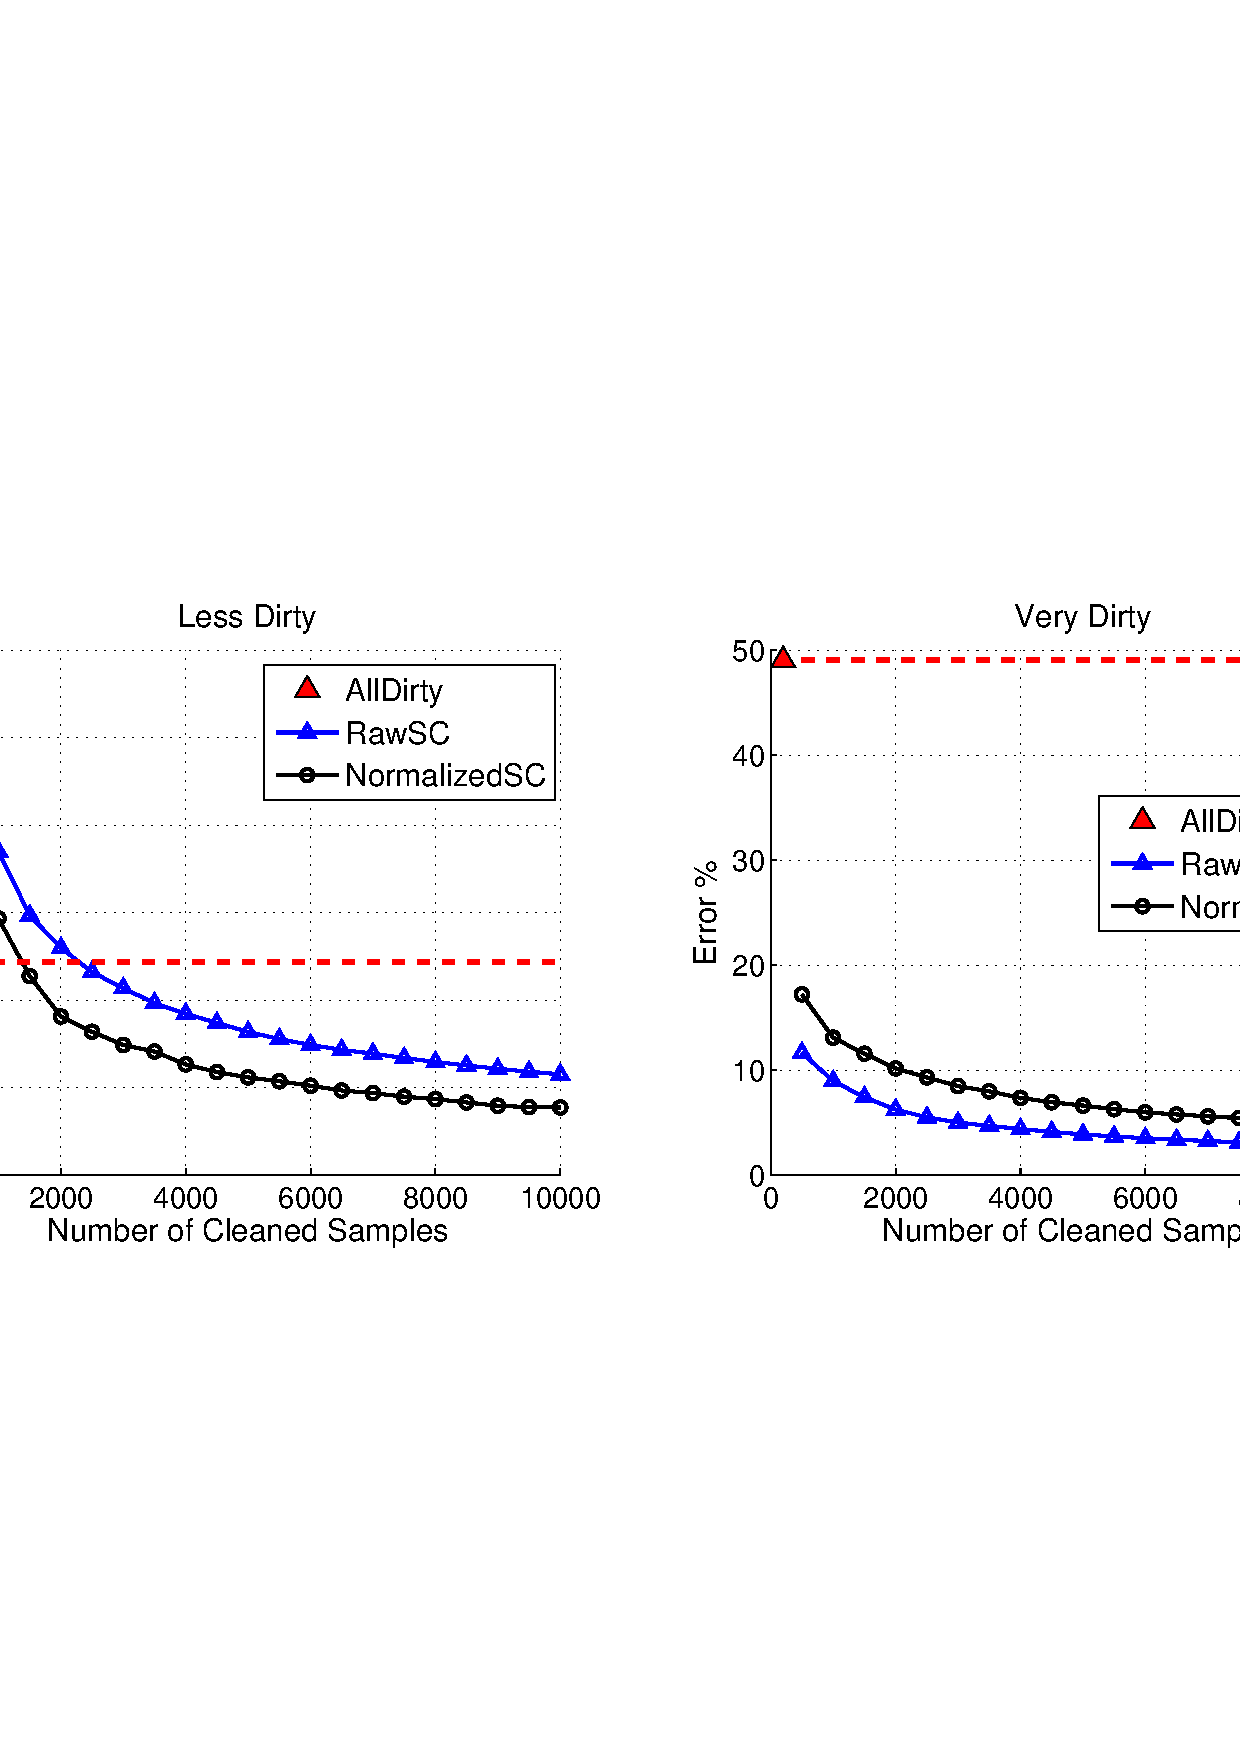
\includegraphics[width=.6\columnwidth]{figs/allerror-samplesize.pdf}
\caption{Comparison of the convergence of the methods on two TPC-H datasets of 6M tuples with simulated errors 50\% error and 5\% error. On the dataset with larger errors, the direct estimate gives a narrower confidence interval, and on the other the correction is more accurate. \label{fig:est2}}
\end{SCfigure}




\section{Problem Statement}
In this section, we formalize the problem explored in this paper.
We are given a set of ER operators,
each of which is a heuristic that is it has some probability of failure or false result.
Furthermore, these probabilities are order dependent.
Ideally, we would like to find the order that minimizes error; however, without ground
truth data this is a difficult objective.
Instead, in this work, we look to find execution orders that are guaranteed not to be too bad.
While not optimal, these can be proven to be close to the expected error the the pipeline.

\subsection{Problem 1. Robust Execution of A Collection of ER Operations}
Given as input a collection of ER operations, and a relation $R$:
\[P = \{\kappa_1, \kappa_2,...,\delta_1,\delta_2\} \]
Let $\mathbb{O}$ be the set of all total orders over P, and $P_o(R)$ be the execution
of the pipeline with a specific total order $o\in \mathbb{O}$.
Let $N(P_o(R))$ be a measure of the error rate of that order of operations.

The output of ESP is some operation $T$ which such that the error rate of applying 
T(R) is close to that of the expected error rate for the pipeline:
\[ \mid N(T(R)) - \mathbb{E}(N(P_o(R))) \mid \le \epsilon w.h.p \ \]

\subsection{Problem 1. Efficient Re-use Of Sub-Pipelines}
\reminder{sort ordering}

\subsection{Problem 3. Correlation Clustering of Multi-Graphs}
\reminder{Multigraph}
\section{Architecture}\label{arch}
This section presents the \sys architecture.

\subsection{Overview}\label{sysover}
Figure \ref{sys-arch} illustrates the \sys architecture.
The dotted boxes describe optional components that the user can supply to improve the efficiency of the system.  

\subsubsection{User Input}\label{uinp}
To use \sys, the user provides the following:

\noindent\textbf{Model:} The user provides a predictive model (e.g., SVM) specified as a convex loss optimization problem $L(\cdot)$ and a featurizer $F(\cdot)$ that maps a record to its feature vector $x$ and label $y$.

\vspace{0.25em}

\noindent\textbf{Cleaning Function: } The data cleaning is specified as a function $C(\cdot)$ that maps dirty records to clean records as per our definition in Section \ref{dmodel}\footnote{\small The record-by-record cleaning model is not a fundamental restriction of this approach, and Appendix~\ref{set-of-r} discusses a compatible ``set of records" cleaning model.
Such a model can capture the case where an analyst finds a dirty record, and can fix all records (possibly outside the sample) the with same error throughout the dataset at a lower cost than cleaning them individually.}.

\vspace{0.25em}

\noindent\textbf{Optional Knobs: } The user can provide two optional hyperparameters.  
A cleaning budget $k$ can be used as a stopping criteria once $C(\dot)$ has been called $k$ times.
A batch size $b$ sets the number of records that are cleaned in each iteration of the ActiveClean algorithm (the number of iterations is $T = \frac{k}{b}$).
Section~\ref{model-update} discusses the efficiency and convergence trade-offs of different values of $b$.

\subsubsection{Data Flow}
The system first trains the model $L(\cdot)$ on the dirty dataset to find an initial model $\theta^(d)$ that the system will subsequently improve.
The {\it Sampler} selects a sample of size $b$ records from the dataset and passes
the sample to the {\it cleaner}, which executes $C(\dot)$ for each sample record and outputs their cleaned versions.
The updater uses the cleaned sample to update the weights of the model, thus moving the model closer to the true cleaned model (in expectation).
Finally, the system either terminates due to a stopping condition (e.g., $C(\dot)$ has been called a maximum number of times $k$, or training error convergence),
or passes control to the {\it Sampler} for the next iteration.

A user provided {\it Detector} can be used to identify records that are more likely to be dirty, and  thus improves the likelihood that the next sample will contain true dirty records.
Furthermore, the {\it Estimator} uses previously cleaned data to estimate the effect that cleaning a given record will have on the model.
These components can be used separately (if only one is supplied) or together to focus the system's cleaning efforts on records that will most improve the model.
Sections \ref{opti} describes several instantiations of these components for different data cleaning problems.

\subsection{Example}

The following illustrates how a user would use \sys in the context of the use case in Section~\ref{s:usecase}:
\begin{example}\label{archex}
\reminder{make story consistent with use case}
The analyst chooses to use an SVM model, and manually clean records by hand (the $C(\dot)$).  
This is enough information for ActiveClean to select a sample of $50$ (the default) records to show the analyst.
She identifies a subset of 15 records that are dirty, fixes them by normalizing the drug and corporation names with the help of a search engine, and improving labels with typographical or incorrect values.
The system then uses the cleaned records to update the model parameters and select the next sample.
The analyst can stop at any time and use the improved model to predict donation likelihoods.
\end{example}






\iffalse
  \noindent To summarize in pseudocode:
  \begin{enumerate}[leftmargin=1em]\scriptsize\sloppy
  \item \texttt{Init(dirty\_data, cleaned\_data, dirty\_model, batch, iter)}
  \item For each t in $\{1,...,T\}$
  \begin{enumerate}
    \item \texttt{dirty\_sample $=$ Sampler(dirty\_data, sample\_prob, detector, batch)}
    \item \texttt{clean\_sample $=$ Cleaner(dirty\_sample)}
    \item \texttt{current\_model $=$ Update(current\_model, sample\_prob, clean\_sample)}
    \item \texttt{cleaned\_data = cleaned\_data + clean\_sample}
    \item \texttt{dirty\_data = dirty\_data - clean\_sample}
    \item \texttt{sample\_prob $=$ Estimator(dirty\_data, cleaned\_data, detector)}
    \item \texttt{detector $=$ DetectorUpdater(detector, cleaned\_data)}
  \end{enumerate}
  \item \texttt{Output: current\_model}
  \end{enumerate}
\fi


\iffalse
  \subsection{Challenges and Formalization}
  We highlight the important components and formalize the research questions explored in this paper. 

  \vspace{0.5em}

  \noindent\textbf{Detector (Section \ref{det}). } The first challenge in \sys is dirty data detection. In this step, the detector selects a candidate set of dirty records $R_{dirty} \subseteq R$. There are two techniques to do this: (1) an \emph{a priori} case, and (2) and an adaptive case. In the \emph{a priori} case, the detector knows which data is dirty in advance. In the adaptive case, the detector learns classifier based on previously cleaned data to detect corruption in uncleaned data.

  \vspace{0.5em}



  \vspace{0.5em}



  \vspace{0.5em}

  \noindent\textbf{Update (Section \ref{model-update}). } This step updates the model $\theta^{(t)}$ based on the featurized (with featurization $F(\cdot)$) cleaned sample $F(S_{clean})$ resulting in $\theta^{(t+1)}$. Analyzing the model update procedure as a stochastic gradient descent algorithm will help derive the sampling distribution and estimation.

  \vspace{0.5em}

  \noindent\textbf{Estimator (Section \ref{sampling}): } The estimator approximates the optimal distribution derived in the Sample step. Based on the change in the featurized data $F(S_{clean})$ and $F(S_{dirty})$, it directs the next iteration of sampling to select points that will have changes most valuable to the next model update.


  \subsection{Optimizations}
  There are three aspects of \sys, that allow us to achieve this design point: error partitioning, gradient-based model update (Section \ref{model-update}), estimate-driven sampling (Section \ref{sampling}).

  \vspace{0.5em}

  \noindent\textbf{Partitioning Dirty and Clean Data: } In many applications, enumerating the set of corrupted records is much easier than cleaning them. For example, we may be able to select the set of rows that have missing values but actually filling those missing values is expensive. Likewise, in the constraint literature, selecting a set of rows that have a violated constraint can be done in polynomial time, however, fixing the constraints is NP-Hard.
  In our error detection step, we partition the dirty and clean data.
  Partitioning serves two purposes: (1) it reduces the variance of our updates because we can cheaply scan over data we know that is clean, and (2) it increases the fraction of actually dirty records in the candidate batch.
  A good example of why we need the second objective is seen in the context of crowdsourcing.
  If we have a crowdworker clean records, we will have to pay them for the task whether or not the record required cleaning.
  To efficiently use this partitioning, we need a database solution indexing dirty and clean data.

  \vspace{0.5em}

  \noindent\textbf{Gradient-Based Updates: } In \sys, we start with a dirty model and then make an update using a gradient step. Here, we can draw an analogy to Materialized View maintenance, since after all, a model parametrized by $\theta$ is just a table of floating point numbers.
  Krishnan et al. proposed a technique called sample view cleaning, in which they take a clean sample of data and propagate the updates to a Materialized View.
  Similarly, in this work, we take the information from a sample of cleaned data and propagate an update with the gradient.

  \vspace{0.5em}

  \noindent\textbf{Estimate-Driven Sampling: } Repair is the most expensive step in the workflow, so optimizing for scan cost may lead to negligible overall time improvements.
  We can sacrifice a small overhead in pre-computation for each data point to determine its value to the model and select a sampling distribution accordingly.
  Intuitively, while each iteration has an increased cost, it also makes more progress towards the optimum.


  \begin{example}\label{archex1}

  The analyst first trains an SVM model on the dirty data ignoring the effects of the errors resulting in a model $\theta^{(d)}$.
  She decides that she has a budget of cleaning $100$ records, and decides to clean the 100 records in batches of 10 (set based on how fast she can clean the data, and how often she wants to see an updated result).
  She initializes \sys with $\theta^{(d)}$.
  \sys samples an initial batch of 10 records.
  She manually cleans those records by merging similar drug names, making corporation names consistent, and fixing incorrect labels.
  After each batch, the model is updated with the most recent cleaning results $\theta^{(t)}$.
  The model improves after each iteration.
  After $t=10$ of cleaning, the analyst has an accurate model trained with 100 cleaned records but still utilizes the entire dirty data.
  \end{example}
\fi



\section{Updates With Correctness}\label{model-update}
This section describes one approach for reliable model updates.
The updater assumes that it is given a sample of data $S_{dirty}$ from $R_{dirty}$ where $i \in S_{dirty}$ has a known sampling probability $p(i)$.
The following sections show how to optimize $p(i)$ and the analysis in this section applies for any sampling distribution $p(\cdot)$.

\subsection{Geometric Derivation}
The update algorithm intuitively follows from the convex geometry of the problem.
Consider this problem in one dimension (i.e., the parameter $\theta$ is a scalar value), so then the goal is to find the minimum point ($\theta$) of a curve $l(\theta)$.
The consequence of dirty data is that the the wrong loss function is optimized.
Figure \ref{update-arch2}A illustrates the consequence of this optimization.
The red dotted line shows the loss function on the dirty data.
Optimizing this loss function finds $\theta$ that at the minimum point (red star).
However, the true loss function (w.r.t to the clean data) is in blue, thus
this optimal value on the dirty data is in fact a suboptimal point on clean curve (red circle).

\begin{figure}[ht!]
\centering
 \includegraphics[width=\columnwidth]{figs/update-arch2.png}\vspace{-1em}
 \caption{(A) A model trained on dirty data can be thought of as a sub-optimal point w.r.t to the clean data. (B) The gradient gives us the direction to move the suboptimal model to approach the true optimum. \label{update-arch2}}\vspace{-1em}
\end{figure}

The optimal clean model $\theta^{(c)}$ is visualized as a yellow star.
The first question is which direction to update $\theta$ (i.e., left or right).
For this class of models, given a suboptimal point, the direction to 
the global optimum is the gradient of the loss function.
The gradient is a $d$-dimensional vector function of the current model $\theta$ and the clean data.
Given this direction, \sys needs to update $\theta^{(d)}$ some distance $\gamma$ (Figure \ref{update-arch2}B):
\[
\theta^{new} \leftarrow \theta^{(d)} - \gamma \cdot \nabla\phi(\theta^{(d)})
\]
At the optimal point, the magnitude of the gradient will be zero.
So intuitively, this approach iteratively moves the model downhill (transparent red circle) -- correcting the dirty model until the desired accuracy is reached.
However, this formulation gradient depends on all of the clean data which is not available and \sys will have to approximate this gradient from a sample.
The main intuition is that if the gradient steps are on average correct, the model still moves downhill albeit with a reduced convergence rate proportional to the inaccuracy of the sample-based estimate.

To derive a sample-based update rule, the most important property is that sums commute with derivatives and gradients.
The convex loss class of models are sums of losses, so given the current best model $\theta$, the gradient $g^*(\theta)$ is:
\[
g^*(\theta) = \nabla\phi(\theta) = \frac{1}{N} \sum_i^N \nabla\phi(x_i^{(c)},y_i^{(c)},\theta)
\]
\sys needs to estimate $g^*(\theta)$ from a sample $S$ is drawn from the dirty data $R_{dirty}$ so this sum has two components the gradient on the already clean data $g_C$ which can be computed without cleaning and $g_S$ the gradient estimate from a sample of dirty data to be cleaned:
\[
g(\theta) = \frac{\mid R_{clean} \mid}{\mid R \mid} \cdot g_C(\theta) + \frac{\mid R_{dirty} \mid}{\mid R \mid} \cdot g_S(\theta)
\]
$g_C$ can be calculated by applying the gradient to all of the already cleaned records:
\[
g_C(\theta) = \frac{1}{\mid R - R_{dirty}\mid}\sum_{i \in R - R_{dirty}}\nabla\phi(x_i^{(c)},y_i^{(c)},\theta)
\]
$g_S$ can be estimated from a sample by taking the gradient w.r.t each record, and re-weighting the average by their respective sampling probabilities.
Before taking the gradient the cleaning function $C(\cdot)$ is applied to each sampled record.
Therefore, let $S$ be a sample of data, where each $i \in S$ is drawn with probability $p(i)$:
\[
g_{S}(\theta) = \frac{1}{\mid S \mid} \sum_{i \in S}\frac{1}{p(i)}\nabla\phi(x_i^{(c)},y_i^{(c)},\theta)
\]
Then, at each iteration $t$, the update becomes:
\[
\theta^{(t+1)} \leftarrow \theta^{(t)} - \gamma \cdot g(\theta^{(t)})
\]

\subsection{Model Update Algorithm}
To summarize, the algorithm is initialized with $\theta^{(1)} = \theta^{(d)}$ which is the dirty model.
There are three user set parameters the budget $k$, batch size $b$, and the step size $\gamma$.
In the following section, we will provide references from the convex optimization literature that allow the user to appropriately select these values.
At each iteration $t=\{1,...,T\}$, the cleaning is applied to a batch of data $b$ selected from the set of candidate dirty records $R_{dirty}$.
Then, an average gradient is estimated from the cleaned batch and the model is updated.
Iterations continue until $k = T \cdot b$ records are cleaned.

\begin{enumerate}[noitemsep]
	\item Calculate the gradient over the sample of clean data and call the result $g_S(\theta^{(t)})$
	\item Calculate the average gradient over all the data in $R_{clean}=R-R_{dirty}$, and call the result $g_C(\theta^{(t)})$
	\item Apply the following update rule:
	\[
	\theta^{(t+1)} \leftarrow \theta^{(t)} - \gamma \cdot(\frac{\mid R_{dirty} \mid}{\mid R \mid} \cdot g_S(\theta^{(t)}) + \frac{\mid R_{clean} \mid}{\mid R \mid} \cdot  g_C(\theta^{(t)}))
	\]
\end{enumerate} 

\subsection{Analysis with Stochastic Gradient Descent}\label{sgd}
This update policy can be formalized as a class of very well studied algorithms called Stochastic Gradient Descent.
This provides a theoretical framework to understand and analyze the update rule and bound the error.
Mini-batch stochastic gradient descent (SGD) is an algorithm for finding the optimal value
given the convex loss and data.
In mini-batch SGD, random subsets of data are selected at each iteration and the average gradient is computed for every batch.

One key difference with traditional SGD models is that \sys applies a \emph{full} gradient step on the already clean data and averages this with a stochastic gradient step (i.e., calculated from a sample) on the dirty data. 
Therefore, \sys iterations can take multiple passes over the clean data but at most a single cleaning pass of the dirty data.
This update method can be thought of as a variant of SGD that lazily materializes the clean value.
As data is sampled at each iteration, data is cleaned when needed by the optimization.
It is well known that even for an arbitrary initialization SGD makes significant progress in less than one epoch (a pass through the entire dataset) \cite{bottou2012stochastic}.
In practice, the dirty model can be much more accurate than an arbitrary initialization as corruption may only affect a few features and combined with the full gradient step on the clean data the updates coverge very quickly.

\vspace{0.25em}

\noindent\textbf{ Setting the step size $\gamma$: } There is extensive literature in machine learning for choosing the step size $\gamma$ appropriately. $\gamma$ can be set either to be a constant or decayed over time. Many machine learning frameworks (e.g., MLLib, Sci-kit Learn, Vowpal Wabbit) automatically set learning rates or provide different learning scheduling frameworks. 
In the experiments, we use a technique called inverse scaling where there is a parameter $\gamma_0=0.1$, and at each iteration it decays to $\gamma_t = \frac{\gamma_0}{\mid S \mid t}$. 

\vspace{0.25em}

\noindent\textbf{ Setting the batch size: } The batch size should be set by the user to have the desired properties.
Larger batches will take longer to clean and will make more progress towards the clean model, but will have less frequent model updates.
On the other hand, smaller batches are cleaned faster and have more frequent model updates but make less progress.
The overheads introduced by \sys are more evident at smaller batch sizes.
There are diminishing returns to increasing the batch size $O(\frac{1}{\sqrt{b}})$.
Empirically, in the experiments, batch sizes of 50 converge the fastest.
If a data cleaning technique requires a larger batch size than this, i.e., data cleaning is fast enough that the iteration overhead is significant compared to cleaning 50 records, \sys can apply the updates in smaller batches.
For example, the batch size set by the user might be $b=1000$, but the model updates after every $50$ records are cleaned.
This dissociates the batching requirements of SGD and the batching requirements of the data cleaning technique.

\subsubsection{Convergence Conditions and Properties}
Convergence properties of batch SGD formulations have been well studied \cite{dekel2012optimal}.Essentially, if the gradient estimate is unbiased and the step size is appropriately chosen, the algorithm is guaranteed to converge. 
In the appendix, we show that the gradient estimate from \sys is indeed unbiased and our choice of step size is one that is established to converge.
The convergence rates of SGD are also well analyzed \cite{dekel2012optimal,bertsekas2011incremental,zhao2014stochastic}. 
This gives a bound on the error of intermediate models and the expected number of steps before achieving a model within a certain error. 
For a general convex loss, a batch size $b$, and $T$ iterations, the convergence rate is bounded by $O(\frac{\sigma^2}{\sqrt{bT}})$. 
$\sigma^2$ is the variance in the estimate of the gradient at each iteration:
\[
\mathbb{E}(\|g_S - g^*\|^2)
\]
If the loss in non-convex, the update procedure will converge towards a local minimum rather than the global minimum (See Appendix \ref{non-convex}).

\subsection{Example}
This example describes an application of the update algorithm.
\begin{example}\label{upex}
Recall that the analyst has a dirty SVM model on the dirty data $\theta^{(d)}$.
She decides that she has a budget of cleaning $100$ records, and decides to clean the 100 records in batches of 10 (set based on how fast she can clean the data, and how often she wants to see an updated result).
All of the data is initially treated as dirty with $R_{dirty} = R$ and $R_{clean} = \emptyset$.
The gradient of a basic SVM is given by the following function:
\[
\nabla\phi(x,y,\theta) =
\begin{cases}      
-y\cdot\boldsymbol{x} \text{ if } y\cdot\boldsymbol{x}\cdot\theta \le 1 \\
0\ \text{ if } y\ \boldsymbol{x}\cdot\theta \geq 1      
\end{cases}
\]

For each iteration $t$, a sample of 10 records $S$ is drawn from $R_{dirty}$.
\sys then applies the cleaning function to the sample:
\[
\{(x_i^{(c)},y_i^{(c)})\} = \{C(i): \forall i \in S\}
\]
Using these values, \sys estimates the gradient on the newly cleaned data:
\[
g_{S}(\theta) = \frac{1}{10} \sum_{i \in S}\frac{1}{p(i)}\nabla\phi(x_i^{(c)},y_i^{(c)},\theta)
\]
\sys also applies this gradient to the already clean data (initially non-existent):
\[
g_C(\theta) = \frac{1}{\mid R_{clean}\mid}\sum_{i \in R - R_{dirty}}\nabla\phi(x_i^{(c)},y_i^{(c)},\theta)
\]
Then, it calculates the update rule:
\[
	\theta^{(t+1)} \leftarrow \theta^{(t)} - \gamma \cdot(\frac{\mid R_{dirty} \mid}{\mid R \mid} \cdot g_S(\theta^{(t)}) + \frac{\mid R_{clean} \mid}{\mid R \mid} \cdot  g_C(\theta^{(t)}))
\] 
Finally, $R_{dirty} \leftarrow R_{dirty} - S$, $R_{clean} \leftarrow R_{clean} + S$, and continue to the next iteration.
\end{example}

\section{Efficiency With Sampling}\label{dist-samp}
The model update received a sample with probabilities $p(\cdot)$.
For any distribution where  $p(\cdot) > 0$, we can preserve correctness.
\sys uses a sampling algorithm that selects the most valuable records to clean with higher probability. 

\subsection{Oracle Sampling Problem}
Recall that the convergence rate of an SGD algorithm is bounded by $\sigma^2$ which is the variance of the gradient.
Intuitively, the variance measures how accurately the gradient is estimated from a uniform sample.
Other sampling distributions, while preserving the sample expected value, may have a lower variance.
Thus, the oracle sampling problem is defined as a search over sampling distributions to find the minimum variance sampling distribution.

\begin{definition}[Oracle Sampling Problem]
Given a set of candidate dirty data $R_{dirty}$, $\forall r \in R_{dirty}$ find sampling probabilities $p(r)$ such that over all samples $S$ of size $k$ it minimizes:
\[
\mathbb{E}(\|g_S - g^*\|^2)
\]
\end{definition}
It can be shown that the optimal distribution over records in $R_{dirty}$ is probabilities proportional to:
\[
p_i \propto \|\nabla\phi(x^{(c)}_i,y^{(c)}_i,\theta^{(t)})\|
\]
We provide proofs and theoretical justification in appendix, but intuitively, records with higher gradients should be sampled with higher probability as they affect the update more significantly.
However, this cannot exclude records with lower gradients as that would induce a bias hurting convergence.
The problem is that this optimal distribution leads to a chicken-and-egg problem:
the optimal sampling distribution requires knowing $(x^{(c)}_i,y^{(c)}_i)$, however, cleaning is required to know those values.

\subsection{Dirty Gradient Solution}
Such an oracle does not exist, and one solution is to use the gradient w.r.t to the dirty data:
\[
p_i \propto \|\nabla\phi(x^{(d)}_i,y^{(d)}_i,\theta^{(t)})\|
\]
It turns out that this solution works reasonably well in practice on our experimental datasets and has been studied in Machine Learning as the Expected Gradient Length heuristic \cite{settles2010active}.
The contribution in this work is integrating this heuristic with statistically valid updates.
However, inutively, approximating the oracle as closely as possible can result in improved priortization.
The subsequent section describes two components, the detector and estimator, that can be used to achieve this.
Our experiments suggest up-to a 2x improvement in convergence when using these optional optimizations (Section \ref{comp}).
\section{Optimizations}\label{opti}


In this section, we describe two approaches to optimization, the {\it Detector} and the {\it Estimator}, that
improve the efficiency of the cleaning process.  
Both approaches are designed to increase the likelihood that the 
{\it Sampler} will pick dirty records that, once cleaned,
most move the model towards the true clean model.
The {\it Detector} is intended to learn the characteristics that distinguish dirty records from clean records
while the {\it Estimator} is designed to estimate the amount that cleaning a given dirty record will move the 
model towards the true optimal model.


\subsection{The Detector}\label{det}
% Partitioning Data With Detection}\label{det}
% \sys improves the progress of each update iteration by intelligently partitioning the data into expected dirty and clean partitions. 
% This ensures that sampling draws data that are likely to be dirty.

% \subsubsection{Goals}
The detector returns two important aspects of a record: 
(1) whether the record is dirty, and (2) if it is dirty, what is wrong with the record.
The sampler can use (1) to select a subset of dirty records to sample at each batch and 
the estimator can use (2) estimate the value of data cleaning based on other records with the same corruption.
\sys supports two types of detectors: \emph{a priori} and \emph{adaptive}.
In former assumes that we know the set of dirty records and how they are dirty \emph{a priori} to \sys,
while the latter \emph{adaptively} learns characteristics of the dirty data as part of running \sys.

\subsubsection{\protect\textit{\large A Priori} Detector}
For many types of dirtiness such as missing attribute values and constraint violations, 
it is possible to efficiently enumerate a set of corrupted records and determine how the records are corrupted.

\begin{definition}[A Priori Detection]
Let $r$ be a record in $R$. An a priori detector is a detector that returns a Boolean of whether the record is dirty and a set of columns $e_r$ that are dirty.
\[
D(r) = (\{0,1\}, e_r)
\]
From the set of columns that are dirty, find the corresponding features that are dirty $f_r$ and labels that are dirty $l_r$.
\end{definition}

\noindent Here are example use cases of this definition using data cleaning methodologies proposed in the literature.

\vspace{0.5em}

\noindent\textbf{Constraint-based Repair: }
One model for detecting errors involves declaring constraints on the database.

\vspace{0.5em}

\emph{Detection. } Let $\Sigma$ be a set of constraints on the relation $\mathcal{R}$. 
In the detection step, the detector selects a subset of records $\mathcal{R}_{dirty} \subseteq \mathcal{R}$ that violate at least one constraint.
The set $e_r$ is the set of columns for each record which have a constraint violation. 

\begin{example}\label{detex1}
An example of a constraint on the running example dataset is that the \texttt{status} of
a contribution can be only ``allowed" or ``disallowed".
Any other value for \texttt{status} is an error.
\end{example}

\subsubsection{Adaptive Detector}
\emph{A priori} detection is not possible in all cases.
The detector also supports adaptive detection where detection is learned from previously cleaned data.
Note that this ``learning" is distinct from the ``learning" at the end of the pipeline.
The challenge in formulating this problem is that detector needs to describe how the data is dirty (e.g. $e_r$ in the \emph{a priori} case).
The detector achieves this by categorizing the corruption into $u$ classes.
These classes are corruption categories that do not necessarily align with features, but every record is classified with at most one category.
For example, suppose there are records with outliers and missing values, there are three classes of corruption: outliers, missing values, and both.

\reminder{Check if it really needs to be combinatorial}
While the number of corruption classes is combinatorial in the individual types, the only classes that need to enumerated are ones that are manifest in the data.
When using adaptive detection, the repair step has to clean the data and report to which of the $u$ classes the corrupted record belongs.
When an example $(x,y)$ is cleaned, the repair step labels it with one of the ${\text{clean}, 1,2,...,u+1}$ classes (including one for ``not dirty").
It is possible that $u$ increases each iteration as more types of dirtiness are discovered. 
Then, the detection problem reduces to a multiclass classification problem.
This problem can be addressed by any multiclass classifier, and we use an all-versus-one SVM in our experiments.

\reminder{Are there different types of adaptive detectors we test?  If so, we should list them out here and talk about tradeoffs/when they are useful!}
\reminder{Also, the learning problem here sounds hopeless (sparse), need to argue why this even makes sense}

\begin{definition}[Adaptive Detection]
Select the set of records for which $\kappa$ gives a positive error classification (i.e., one of the $u$ error classes).
After each sample of data is cleaned, the classifier $\kappa$ is retrained.
So the result is:
\[D(r) = (\{1,0\},\{1,...,u+1\})\]
\end{definition}

\vspace{0.75em}

\noindent\textbf{Adaptive Detection With OpenRefine: }
\begin{example}\label{detex2}
OpenRefine is a spreadsheet-based tool that allows users to explore and transform data.
However, it is limited to cleaning data that can fit in memory on a single computer.
Since the cleaning operations are coupled with data exploration, \sys does not know what is dirty in advance (the analyst may discover new errors as she cleans).

Suppose the analyst wants to use OpenRefine to clean the running example dataset with \sys.
She takes a sample of data from the entire dataset and uses the tool to discover errors.
For example, she finds that some drugs are incorrectly classified as both drugs and devices.
She then removes the device attribute for all records that have the drug name in question.
As she fixes the records, she tags each one with a category tag of which corruption it belongs to.
\end{example}








\subsection{The Estimator}\label{sampling}
%\subsubsection{Approximating an Oracle Sampler}
To get around the problem with oracle sampling, the estimator will estimate the cleaned value with previously cleaned data.
The estimator will also take advantage of the detector from the previous section.
There are a number of different approaches, such as regression, that could be used to estimate the cleaned value given the dirty values.
However, there is a problem of scarcity, where errors may affect a small number of records.
As a result, the regression approach would have to learn a multivariate function with only a few examples.
This makes high-dimensional regression ill-suited for the estimator.
Conversely, it could try a very simple estimator that just calculates an average change and adds this change to all of the gradients.
This estimator can be highly inaccurate as it also applies the change to records that are known to be clean.

\sys leverages the detector for an estimator that is in between these two extremes.
The estimator calculates average changes feature-by-feature and selectively corrects the gradient when a feature is known to be corrupted based on the detector.
It also applies a linearization that leads to improved estimates when the sample size is small.
We evaluate this linearization in Section \ref{est} against alternatives, and find that it provides more accurate estimates for a small number of samples cleaned.
This is a biased estimator, and when the number of cleaned samples is large the alternative techniques are comparable or even slightly better due to the bias.

\paragraph{Estimation For A Priori Detection}
If most of the features are correct, it would seem like the gradient is only
incorrect in one or two of its components.
The problem is that the gradient $\nabla\phi(\cdot)$ can be a very non-linear function of the features that couple features together.
For example, the gradient for linear regression is:
\[
\nabla\phi(x,y,\theta) = (\theta^Tx - y)x
\]
It is not possible to isolate the effect of a change of one feature on the gradient.
Even if one of the features is corrupted, all of the gradient components will be incorrect.

To address this problem, the gradient can be approximated in a way that the effects of dirty features on the gradient are decoupled.
Recall, in the \emph{a priori} detection problem, that associated with each $r \in R_{dirty}$ is a set of errors $f_r,l_r$ which is a set that identifies a set of corrupted features and labels.
This property can be used to construct a coarse estimate of the clean value.
The main idea is to calculate average changes for each feature, then given an uncleaned (but dirty) record, add these average changes to correct the gradient.

To formalize this intuition, instead of computing the actual gradient with respect to the 
true clean values, compute the conditional expectation given that a set of features and labels $f_r,l_r$ are corrupted:
\[
p_i \propto \mathbb{E}(\nabla\phi(x^{(c)}_i,y^{(c)}_i,\theta^{(t)}) \mid f_r,l_r)
\]
Corrupted features are defined as that:
\[
i \notin f_r \implies x^{(c)}[i] - x^{(d)}[i] = 0
\]
\[
i \notin l_r \implies y^{(c)}[i] - y^{(d)}[i] = 0
\]

The needed approximation represents a linearization of the errors, and the resulting approximation will be of the form:
\[
p(r)\propto\|\nabla\phi(x,y,\theta^{(t)}) + M_x \cdot \Delta_{rx} +  M_y \cdot \Delta_{ry}\|
\]
where $M_x$, $M_y$ are matrices and $\Delta_{rx}$ and $\Delta_{ry}$ are vectors with one component for each feature and label where each value is the average change for those features that are corrupted and 0 otherwise.
Essentially, it the gradient with respect to the dirty data plus some linear correction factor.
In the appendix, we present a derivation using a Taylor series expansion and a number of $M_x$ and $M_y$ matrices for common convex losses.
The appendix also describes how to maintain $\Delta_{rx}$ and $\Delta_{ry}$ as cleaning progresses.

\iffalse
\paragraph{More Accurate Early Error Estimates}\label{acc}
Linearization over avoids amplifying estimation error.
Consider the linear regression gradient:
\[
\nabla\phi(x,y,\theta) = (\theta^Tx - y)x
\]
This can be rewritten as a vector in each component:
\[
g[i] = \sum_{i} x[i]^2-x[i]y + \sum_{j \ne i} \theta[j]x[j]
\]
This function is already mostly linear in $x$ except for the one quadratic term.
However, this one quadratic term has potential to amplify errors.
Consider two expressions:
\[
f(x+\epsilon) = (x+\epsilon)^2 = x^2 + 2x\epsilon + \epsilon^2
\]
\[
f(x+\epsilon) \approx f(x) + f'(x)(\epsilon) = x^2 + 2x\epsilon
\]
The only difference between the two estimates is the quadratic $\epsilon^2$, if $\epsilon$ is highly uncertain random variable then the quadratic dominates.
If this variance is large, the Taylor estimate avoids amplifying this error.
Of course, this is at the tradeoff of some additional bias since the true function is non-linear.
We evaluate this linearization in Section \ref{est} against alternatives, and find that indeed it provides more accurate estimates for a small number of samples cleaned.
When the number of cleaned samples is large the alternative techniques are comparable or even slightly better.
\fi

\paragraph{Estimation For Adaptive Case}
A similar procedure holds in the adaptive setting, however, it requires reformulation.
Here, \sys uses $u$ corruption classes provided by the detector.
Instead of conditioning on the features that are corrupted, the estimator conditions on the classes.
So for each error class, it computes a $\Delta_{ux}$ and $\Delta_{uy}$.
These are the average change in the features given that class and the average change in labels given that class.
\[
p(r_u)\propto\|\nabla\phi(x,y,\theta^{(t)}) + M_x \cdot \Delta_{ux} +  M_y \cdot \Delta_{uy}\|
\] 

\subsubsection{Example}
Here is an example of using the optimization to select a sample of data for cleaning.
\begin{example}
Consider using \sys with an a priori detector.
Let us assume that there are no errors in the labels and only errors in the features.
Then, each training example will have a set of corrupted features (e.g., $\{1,2,6\}$, $\{1,2,15\}$).
Suppose that the cleaner has just cleaned the records $r_1$ and $r_2$ represented as tuples with their corrupted feature set: ($r_1$,$\{1,2,3\}$), ($r_2$,$\{1,2,6\}$).
For each feature $i$, \sys maintains the average change between dirty and clean in a value in a vector $\Delta_x[i]$ for those records corrupted on that feature. 

Then, given a new record ($r_3$,$\{1,2,3,6\}$), $\Delta_{r_3x}$ is the vector $\Delta_x$ where component $i$ is set to 0 if the feature is not corrupted.
Suppose the data analyst is using an SVM, then the $M_x$ matrix is as follows:
\[
M_x[i,i] = \begin{cases}      
-y[i] \text{ if } y\cdot\boldsymbol{x}\cdot\theta \le 1 \\
0\ \text{ if } y\ \boldsymbol{x}\cdot\theta \geq 1      
\end{cases} 
\]
Thus, we calculate a sampling weight for record $r_3$:
\[
p(r_3) \propto\|\nabla\phi(x,y,\theta^{(t)}) + M_x \cdot \Delta_{r_3x} \|
\] 
To turn this into a probability, \sys normalizes over all dirty records.
\end{example}




% \input{detect.tex}

% \input{impestimate.tex}

%\section{Adaptive Error Detection}\label{imperfect} 
In this section, we explore how we can handle the case where the error detection is learned as we clean data.

\subsection{Challenges}
In this section, we explore the partitioning model, where as we clean more data, we iteratively prune data we expect to be clean from $R_{dirty}$.
This is done with a classifier that is updated with new training data based on the previous iterations results.
The main challenge is that the sampling weights calculated in the previous section are dependent on the error detection step returning a set of corrupted features.
When we relax this assumption, there are new challenges in error estimation.
Next, an important aspect of our gradient update is partitioning the dirty and clean data.
We aggregate an average gradient from both subpopulations when making our update.
However, in some cases, characterizing this partioning can be difficult and it may be impossible to ensure this condition unless $R_{dirty} = R$ causing a loss in efficiency if errors are sparse. 

\subsection{Error Classes}
When we relax the restrictions on the error detection step, we no long have a set of corrupted features $e_r$.
This breaks the decoupling argument that we made in the previous section.
However, our high-level goal in the previous section, was to estimate the gradient for groups of similarly corrupted records.
We try to formulate an analogous methodology that generalizes what we did in the previous section to error detection steps that are learned over time.
Instead of assuming that we know which features are corrupted, let us say that we know that there are $u$ classes of errors.
As the analyst cleans data, she tags dirty data with one of the $u$ classes.
Then, the error detection problem reduces to a multiclass classification problem.
Once classified, we can apply an average change conditioned on the error class.

With this intuition in mind, we have to revise our error repair step:
\vspace{0.5em}

\noindent\textbf{Error Repair: } When an example $(x,y)$ is cleaned, the repair step also has to provide a label of to which of the ${\text{clean}, 1,2,...,u}$ classes it belongs. It is possible that $u$ increases each iteration as more errors are discovered. 

\vspace{0.5em}

Suppose, we have a multi-class classifier $\kappa$ (e.g. SVM) that classifies every record $r$ into $u+1$ classes (the $u$ error types or not dirty).
Thus, we revise the partitioning in the following way:

\vspace{0.5em}

\noindent\textbf{Error Detection: } To select $R_{dirty}$, we select the set of records for which $\kappa$ give a positive error classification (i.e., one of the $u$ error classes).
Many types of classifiers allow users to tradeoff precision and recall.
In other words, we can also select any record within some level of confidence of the classification margin.
For an SVM, we may only classify a point as clean if it is sufficiently far from the margin.
Or for Logistic Regression, we may do so if its class likelihood is over 80\%.

\subsection{Error Estimate}
Our model update framework still holds in this setting, however, our error estimation framework requires some modification.
In our derivation, we showed that our error estimate was a linearization of the conditional expectation of the gradient.
Instead of conditioning on the features that are corrupted, we condition the error classes.
So for each error class, we compute a $\Delta_{xu}$ and $\Delta_{yu}$.
These are the average change in the features given that class and the average change in labels given that class respectively.
\[
p_{r,u}\propto\|\nabla\phi(x,y,\theta^{(t)}) + M_x \cdot \Delta_{ux} +  M_y \cdot \Delta_{uy}\|
\] 



\section{Experiments}\label{eval}
First, the experiments evaluate how various types of corrupted data benefit from data cleaning.
Next, the experiments explore different prioritization and model update schemes for progressive data cleaning.
Finally, \sys is evaluated end-to-end in a number of real-world data cleaning scenarios.

\subsection{Experimental Setup and Notation}
The main metric for evaluation is a relative measure of the trained model and the model if all of the data is cleaned.

\vspace{0.5em}

\noindent\textbf{Relative Model Error. } Let $\theta$ be the model trained on the dirty data, and let $\theta^*$ be the model trained on the same data if it was cleaned. Then the model error is defined as $\frac{\|\theta - \theta^*\|}{\|\theta^*\|}$.

\subsubsection{Scenarios}
%\vspace{0.5em}

%\noindent\textbf{Housing: } In this dataset, our task is to predict housing prices from 13 numerical and categorical covariates. There are 550 data points in this dataset. The model is a Logistic Regression classifier which predicts if the house price is greater than \$500k.

\vspace{0.25em}

\noindent\textbf{Income Classification (Adult): } In this dataset of 45,552 records, the task is to predict the income bracket (binary) from 12 numerical and categorical covariates with an SVM classifier. 

\vspace{0.25em}

\noindent\textbf{Seizure Classification (EEG): } In this dataset, the task is to predict the onset of a seizure (binary) from 15 numerical covariates with a thresholded Linear Regression. There are 14980 data points in this dataset. This classification task is inherently hard with an accuracy on completely clean data of only 65\%.

\vspace{0.25em}

\noindent\textbf{Handwriting Recognition (MNIST) \footnote{\scriptsize\url{http://ufldl.stanford.edu/wiki/index.php/Using_the_MNIST_Dataset}}: } In this dataset, the task is to classify 60,000 images of handwritten images into 10 categories with an one-to-all multiclass SVM classifier. The unique part of this dataset is the featurized data consists of a 784 dimensional vector which includes edge detectors and raw image patches. 

\vspace{0.25em}

\noindent\textbf{Dollars For Docs: } The dataset has 240,089 records with 5 textual attributes and one numerical attribute.
The dataset is featurized with bag-of-words featurization model for the textual attributes which resulted in a 2021 dimensional feature vector, and a binary SVM is used to classify the status of the medical donations.

\subsubsection{Compared Algorithms}
\noindent Here are the alternative methodologies evaluated in the experiments:

\vspace{0.25em}

\noindent\textbf{Robust Logistic Regression \cite{feng2014robust}. } Feng et al. proposed a variant of logistic regression that is robust to outliers. We chose this algorithm because it is a robust extension of the convex regularized loss model, leading to a better apples-to-apples comparison between the techniques. (See details in Appendix \ref{rlogit})  

\vspace{0.25em}

\noindent\textbf{Discarding Dirty Data. } As a baseline, dirty data is discarded.

\vspace{0.25em}

\noindent\textbf{SampleClean (SC) \cite{wang1999sample}. } SampleClean takes a sample of data, applies data cleaning, and then trains a model to completion on the sample.

\vspace{0.25em}

\noindent\textbf{Active Learning (AL) \cite{guillory2009active}. } An Active Learning algorithm that integrates with stochastic optimization (See details in Appendix \ref{al}). 

\vspace{0.25em}

\noindent\textbf{ActiveClean Oracle (AC+O): } In \sys Oracle, instead of an estimation step, the true clean value is used to evaluate the theoretical ideal performance of \sys.

\subsection{Does Data Cleaning Matter?}
The first experiment evaluates the benefits of data cleaning on two of the example datasets (EEG and Adult).
This is done without sampling to understand which types of data corruption are amenable to data cleaning and which are better suited for robust statistical techniques.
The experiment compares four schemes: (1) full data cleaning  , (2) baseline of no cleaning, (3) discarding the dirty data, and (4) robust logistic regression,. We corrupted 5\% of the training examples in each dataset in two different ways:

\vspace{0.5em}

\noindent\textbf{Random Corruption: } Simulated high-magnitude random outliers. 5\% of the examples are selected at random and a random feature is replaced with 3 times the highest feature value.

\vspace{0.5em}

\noindent\textbf{Systematic Corruption: } Simulated innocuous looking (but still incorrect) systematic corruption. The model is trained on the clean data, and the three most important features (highest weighted) are identified. The examples are sorted by each of these features and the top examples are corrupted with the mean value for that feature (5\% corruption in all). 
It is important to note that examples can have multiple corrupted features.

\begin{figure}[t]
\centering
 \includegraphics[width=0.49\columnwidth]{exp/exp2.pdf}
 \includegraphics[width=0.49\columnwidth]{exp/exp1.pdf}
 \includegraphics[width=0.5\columnwidth]{exp/legend-1.png}\vspace{-1em}
 \caption{(a) Robust techniques and discarding data work when corrupted data are random and look atypical. (b) Data cleaning can provide reliable performance in both the systematically corrupted setting and randomly corrupted setting.\label{sys-rand}}\vspace{-1.5em}
\end{figure}

Figure \ref{sys-rand} shows the test accuracy for models trained on both types of data with the different techniques.
The robust method performs well on the random high-magnitude outliers with only a 2.0\% reduction in clean test accuracy for EEG and 2.5\% reduction for Adult.
In the random setting, discarding dirty data also performs relatively well.
However, the robust method falters on the systematic corruption with a 9.1\% reduction in clean test accuracy for EEG and 10.5\% reduction for Adult.
%Data cleaning is the most reliable option across datasets and corruption types.
The problem is that without cleaning, there is no way to know if the corruption is random or systematic and when to trust a robust method.
While data cleaning requires more effort, it provides benefits in both settings.
In the remaining experiments, unless otherwise noted, the experiments use systematic corruption.

\noindent \emph{Summary: A 5\% systematic corruption can introduce a 10\% reduction in test accuracy even when using a robust method.}

\subsection{\sys: \protect\textit{\large A Priori} Detection}
The next set of experiments evaluate different approaches to cleaning a sample of data compared to \sys using \emph{a priori} detection.
\emph{A priori} detection assumes that all of the corrupted records are known in advance but their clean values are unknown. 

\subsubsection{Active Learning and SampleClean}
The next experiment evaluates the samples-to-error tradeoff between four alternative algorithms: \sys (AC), SampleClean, Active Learning, and \sys+Oracle (AC+O).
Figure \ref{prio-perf} shows the model error and test accuracy as a function of the number of cleaned records.
In terms of model error, \sys gives its largest benefits for small sample sizes.
For 500 cleaned records of the Adult dataset, \sys has 6.1x less error than SampleClean and 2.1x less error than Active Learning.
For 500 cleaned records of the EEG dataset, \sys has 9.6x less error than SampleClean and 2.4x less error than Active Learning.
Both Active Learning and \sys benefit from the initialization with the dirty model as they do not retrain their models from scratch, and \sys improves on this performance with detection and error estimation.
Active Learning has no notion of dirty and clean data, and therefore prioritizes with respect to the dirty data.
These gains in model error also correlate well to improvements in test error (defined as the test accuracy difference w.r.t cleaning all data).
The test error converges more quickly than model error, emphasizing the benefits of progressive data cleaning, since it is not neccessary to clean all the data to get a model with essentially the same performance as the clean model.
For example, to achieve a test error of 1\% on the Adult dataset, \sys cleans 500 fewer records than Active Learning.


\vspace{0.25em}

\noindent \emph{Summary: \sys with a priori detection returns results that are more than 6x more accurate than SampleClean and 2x more accurate than Active Learning for cleaning 500 records.}

\begin{figure}[t]
\centering\vspace{-1em}
 %\includegraphics[scale=0.15]{exp/exp3a.pdf}
 \includegraphics[width=0.49\columnwidth]{exp/exp3b.pdf}
  \includegraphics[width=0.49\columnwidth]{exp/exp3c.pdf}
  \includegraphics[width=0.49\columnwidth]{exp/exp3bb.pdf}
  \includegraphics[width=0.49\columnwidth]{exp/exp3cc.pdf}
  \includegraphics[width=0.5\columnwidth]{exp/legend-general.png}\vspace{-0.5em}
 \caption{ The relative model error as a function of the number of examples cleaned. \sys converges with a smaller sample size to the true result in comparison to Active Learning and SampleClean. \label{prio-perf}}\vspace{-1em}
\end{figure}

\subsubsection{Source of Improvements}\label{comp}
The next experiment compares the performance of \sys with and without various optimizations at 500 records cleaned point. 
This is a vertical slice of the plots in the previous experiments.
\sys without detection is denoted as (AC-D) (that is at each iteration we sample from the entire dirty data), and \sys without detection and importance sampling is denoted as (AC-D-I).
Figure \ref{opts} plots the relative error of the alternatives and \sys with and without the optimizations.
Without detection (AC-D), \sys is still more accurate than Active Learning.
Removing the importance sampling, \sys is slightly worse than Active Learning on the Adult dataset but is comparable on the EEG dataset.

\begin{figure}[t]\vspace{0.5em}
\centering
 \includegraphics[width=0.49\columnwidth]{exp/exp8a.png}
 \includegraphics[width=0.49\columnwidth]{exp/exp8b.png}
 \includegraphics[width=0.5\columnwidth]{exp/legend-8.png}\vspace{-1em}
 \caption{ -D denotes no detection, and -D-I denotes no detection and no importance sampling. Both optimizations significantly help \sys outperform SampleClean and Active Learning. \label{opts}}\vspace{-1.5em}
\end{figure}

\vspace{0.25em}

\noindent \emph{Summary: Both a priori detection and non-uniform sampling significantly contribute to the gains over Active Learning.}

\iffalse
We evaluate Active Learning and \sys to better understand this relationship.
In Figure \ref{albias}, we vary the biasing effect of the random corruptions.
That is, we start with zero mean noise and increase the mean value and variance of the noise.
Since Active Learning uses the gradient, if there is zero mean noise, in expectation, the dirty data and clean data are the same.
However, as the bias increases, the fact that Active Learning prioritizes w.r.t to the dirty data matters more and becomes increasingly erroneous w.r.t to \sys.

\begin{figure}[ht!]
\centering
 \includegraphics[width=0.6\columnwidth]{exp/exp10.pdf}
 \caption{As we increase the biasing nature of the corruption, Active Learning is increasingly erroneous w.r.t \sys. \label{albias}}
\end{figure}
\fi

\subsubsection{Mixing Dirty and Clean Data}
Training a model on mixed data is an unreliable methodology lacking the same guarantees as Active Learning or SampleClean even in the simplest of cases.
For thoroughness, the next experiments include the model error as a function of records cleaned in comparison to \sys.
Figure \ref{pc-perf} plots the same curves as the previous experiment comparing \sys, Active Learning, and two mixed data algorithms.
PC randomly samples data, clean, and writes-back the cleaned data.
PC+D randomly samples data from using the dirty data detector, cleans, and writes-back the cleaned data.
For these errors PC and PC+D give reasonable results (not always guaranteed), but \sys converges faster.
This is because \sys tunes the weighting when averaging dirty and clean data into the gradient.

\begin{figure}[ht!]
\centering\vspace{-0.5em}
 %\includegraphics[scale=0.15]{exp/exp3a.pdf}
 \includegraphics[width=0.49\columnwidth]{exp/exp14a.pdf}
    \includegraphics[width=0.49\columnwidth]{exp/exp14b.pdf}
    \includegraphics[width=0.49\columnwidth]{exp/legend-14.png}\vspace{-0.5em}
 \caption{The relative model error as a function of the number of examples cleaned. \sys converges with a smaller sample size to the true result in comparison to partial cleaning (PC,PC+D).  \label{pc-perf}}
\end{figure}

\noindent \emph{Summary: \sys converges faster than mixing dirty and clean data since it reweights data based on the fraction that is dirty and clean. Partial cleaning is not guaranteed to give sensible results.}

\vspace{1em}

\subsubsection{Corruption Rate}
The next experiment explores how much of the performance
is due to the initialization with the dirty model (i.e., SampleClean trains a model from ``scratch").
Figure \ref{bias} varies the systematic corruption rate and plots the number of records cleaned to achieve 1\% relative error for SampleClean and \sys.
SampleClean does not use the dirty data and thus its error is essentially governed by the Central Limit Theorem.
SampleClean outperforms \sys only when corruptions are very severe (45\% in Adult and nearly 60\% in EEG).
When the initialization with the dirty model is inaccurate, \sys does not perform as well. 

\begin{figure}[t]
\centering
 \includegraphics[width=0.49\columnwidth]{exp/exp9a.pdf}
  \includegraphics[width=0.49\columnwidth]{exp/exp9b.pdf}\vspace{-1em}
 \caption{\sys performs well until the corruption is so severe that the dirty model is not a good initialization. The error of SampleClean does not depend on the corruption rate so it is a vertical line.  \label{bias}}\vspace{-1.5em}
\end{figure}

\vspace{0.25em}

\noindent \emph{Summary: SampleClean is beneficial in comparison to \sys when corruption rates exceed 45\%.}

\subsection{\sys: Adaptive Detection}
This experiment explores how the results of the previous experiment change when using an adaptive detector instead of the \emph{a priori} detector.
Recall, in the systematic corruption, 3 of the most informative features were corrupted, thus we group these problems into $9$ classes.
We use an all-versus-one SVM to learn the categorization.

\subsubsection{Basic Performance}
Figure \ref{pred-perf} overlays the convergence plots in the previous experiments with a curve (denoted by AC+C) that represents \sys using a classifier instead of the \emph{a priori} detection. Initially \sys is comparable to Active Learning; however, as the classifier becomes more effective the detection improves the performance.
Over both datasets, at the 500 records point on the curve, adaptive \sys has a 30\% higher model error compared to \emph{a priori} \sys.
At 1000 records point on the curve, adaptive \sys has about 10\% higher error.

\vspace{0.25em}

\noindent \emph{Summary: For 500 records cleaned, adaptive \sys has a 30\% higher model error compared to a priori \sys, but still outperforms Active Learning and SampleClean.}

\begin{figure}[ht!]
\centering
 \includegraphics[width=0.49\columnwidth]{exp/exp11a.pdf}
 \includegraphics[width=0.49\columnwidth]{exp/exp11b.pdf}
 \includegraphics[width=0.49\columnwidth]{exp/legend-11.png}\vspace{-0.5em}
 \caption{Even with a classifier \sys converges faster than Active Learning and SampleClean. \label{pred-perf}}\vspace{-1.0em}
\end{figure}


\subsubsection{Classifiable Errors}
The adaptive case depends on being able to predict corrupted records.
For example, random corruption not correlated with any other data features may be hard to learn.
As corruption becomes more random, the classifier becomes increasingly erroneous.
The next experiment explores making the systematic corruption more random.
Instead of selecting the highest valued records for the most valuable features, we corrupt random records with probability $p$. 
We compare these results to AC-D where we do not have a detector at all at one vertical slice of the previous plot (cleaning 1000 records).
Figure \ref{tradeoffs2}a plots the relative error reduction using a classifier.
When the corruption is about 50\% random then there is a break even point where no detection is better.
This is because the classifier is imperfect and misclassifies some data points incorrectly as cleaned.

\vspace{0.25em}

\noindent \emph{Summary: When errors are increasingly random (50\% random) and cannot be accurately classified, adaptive detection provides no benefit over no detection. }

\begin{figure}[ht!]
\centering \vspace{-1em}
 \includegraphics[width=0.49\columnwidth]{exp/exp5a.pdf}
 \includegraphics[width=0.49\columnwidth]{exp/exp12.pdf}\vspace{-0.5em}
 \caption{(a) Data corruptions that are less random are easier to classify, and lead to more significant reductions in relative model error. (b) The Taylor series approximation gives more accurate estimates when the amount of cleaned data is small. \label{tradeoffs2}}\vspace{-2em}
\end{figure}

\vspace{1.5em}
\subsection{Estimation}\label{est}
The next experiment compares estimation techniques: (1) ``linear regression" trains a linear regression model that predicts the clean gradient as a function of the dirty gradient, (2) ``average gradient" which does not use the detection to inform how to apply the estimate, (3) ``average feature change" uses detection but no linearization, and (4) the Taylor series linear approximation.
Figure \ref{tradeoffs2}b measures how accurately each estimation technique estimates the gradient as a function of the number of cleaned records on the EEG dataset.

Estimation error is measured using the relative L2 error with the true gradient.
The Taylor series approximation proposed gives more accurate for small cleaning sizes, confirming the analysis in Section \ref{acc}.
Linear regression and the average feature change technique do eventually perform comparably but only after cleaning much more data.

\vspace{0.25em}

\noindent \emph{Summary: Linearized gradient estimates are more accurate when estimated from small samples. }

\subsection{Real World Scenarios}
The next set of experiments evaluate \sys in two real world scenarios, one demonstrating the \emph{a priori} case and the other for the adaptive detection case.

\subsubsection{A Priori: Constraint Cleaning}\label{dfd-exp}
The first scenario explores the Dollars for Docs dataset published by ProPublica described throughout the paper.
To run this experiment, the entire dataset was cleaned up front, and simulated sampling from the dirty data and cleaning by looking up the value in the cleaned data (see Appendix \ref{dfd-errors} for constraints, errors, and cleaning methodology).
Figure \ref{dfd}a shows that \sys converges faster than Active Learning and SampleClean.
To achieve a 4\% relative error (i.e., a 75\% error reduction from the dirty model), \sys cleans 40000 fewer records than Active Learning.
Also, for 10000 records cleaned, \sys has nearly an order of magnitude smaller error than SampleClean.

Figure \ref{dfd}b shows the detection rate (fraction of disallowed research contributions identified) of the classifier as a function of the number of records cleaned. 
On the dirty data, we can only correctly classify 66\% of the suspected examples (88\% overall accuracy due to a class imbalance).
On the cleaned data, this classifier is nearly perfect with a 97\% true positive rate (98\% overall accuracy).
\sys converges to the cleaned accuracy faster than the alternatives with a classifier of 92\% true positive rate for only 10000 records cleaned.

\vspace{0.25em}

\noindent \emph{Summary: To achieve an 80\% detection rate, \sys cleans nearly 10x less records than Active Learning. }

\begin{figure}[t]
\centering\vspace{-1em}
 \includegraphics[width=0.49\columnwidth]{exp/exp13a.pdf}
 \includegraphics[width=0.49\columnwidth]{exp/exp13b.pdf}\vspace{-1em}
 \caption{(a) The relative model error as a function of the number of cleaned records. (b) The true positive rate as a function of the number of cleaned records. \label{dfd}}
\end{figure}

\subsubsection{Adaptive: Replacing Corrupted Data}
The next experiment explores the MNIST handwritten digit recognition dataset with a MATLAB image processing pipeline.
In this scenario, the analyst must inspect a potentially corrupted image and replace it with a higher quality one.
The MNIST dataset consists of 64x64 grayscale images.
There are two types of simulated corruptions: (1) 5x5 block removal where a random 5x5 block is removed from the image by setting its pixel values to 0, and (2) Fuzzy where a 4x4 moving average patch is applied over the entire image.
These corruptions are applied to a random 5\% of the images, and mimic the random (Fuzzy) vs. systematic corruption (5x5 removal) studied in the previous experiments.
The adaptive detector uses a 10 class classifier (one for each digit) to detect the corruption.

Figure \ref{mnist} shows that \sys makes more progress towards the clean model with a smaller number of examples cleaned.
To achieve a 2\% error for the block removal, \sys can inspect 2200 fewer images than Active Learning and 2750 fewer images than SampleClean.
For the fuzzy images, both Active Learning and \sys reach 2\% error after cleaning fewer than 100 images, while SampleClean requires 1750.

\vspace{0.25em}

\noindent \emph{Summary: In the MNIST dataset, \sys significantly reduces (more than 2x) the number of images to clean to train a model with 2\% error. }

\begin{figure}[t]
\centering
 \includegraphics[width=0.49\columnwidth]{exp/exp7a.pdf}
 \includegraphics[width=0.49\columnwidth]{exp/exp7b.pdf}
 \includegraphics[width=0.49\columnwidth]{exp/legend-general.png}\vspace{-0.5em}
 \caption{In a real adaptive detection scenario with the MNIST dataset, \sys outperforms Active Learning and SampleClean.  \label{mnist}}\vspace{-1em}
\end{figure}


\vspace{-1em}
\section{Related Work}\label{sec:rw}
{\noindent \bf Approximate Query Processing:} \saqp has been studied for more than two decades~\cite{DBLP:conf/vldb/GarofalakisG01,DBLP:journals/ftdb/CormodeGHJ12}.
Many \saqp approaches~\cite{DBLP:journals/tods/ChaudhuriDN07,DBLP:conf/eurosys/AgarwalMPMMS13,DBLP:conf/sigmod/AcharyaGPR99,DBLP:conf/cidr/SidirourgosKB11,DBLP:conf/sigmod/BabcockCD03,DBLP:conf/sigmod/HellersteinHW97,DBLP:journals/pvldb/PansareBJC11,DBLP:conf/sigmod/CondieCAHGTES10,DBLP:journals/pvldb/WuJOT09} were proposed, aiming to enable interactive query response times.
%Acharya et al.~\cite{DBLP:conf/sigmod/AcharyaGPR99} developed the Aqua system which is run on top of relational DBMS, and allows users to obtain approximate query answers in a fast response time. Chaudhuri et al.~\cite{DBLP:journals/tods/ChaudhuriDN07} studied how to create an optimal stratified random sample based on a given query workload, and proposed the STRAT algorithm that can make the workload queries achieve the best quality on the sample. Sidirourgos et al.~\cite{DBLP:conf/cidr/SidirourgosKB11} presented the SciBORQ architecture that creates biased multi-layered samples based on the scientific data exploration workload, and adaptively select a suitable sample to satisfy quality or time constraints during query execution. Agarwal et al.~\cite{DBLP:conf/eurosys/AgarwalMPMMS13} devised novel multi-dimensional stratified samples based on real-world big data analytics workloads, and built the BlinkDB system to utilize the created samples to support interactive query processing with error and response time constraints. Unlike the above approaches which create samples ahead of query time, online aggregation~\cite{DBLP:conf/sigmod/HellersteinHW97,DBLP:journals/pvldb/PansareBJC11,DBLP:conf/sigmod/CondieCAHGTES10,DBLP:journals/pvldb/WuJOT09} constructs samples in an online fashion, and gradually achieve more and more accurate results until users are satisfied about the current results. 
There are also many studies on creating other synopsis of the data, such as histograms or wavelets~\cite{DBLP:journals/ftdb/CormodeGHJ12}. While a substantial works on approximate query processing, these works mainly focus on how to deal with sampling errors, with little attention to data errors. 

\vspace{.5em}

{\noindent \bf Data Cleaning:} There have been many studies on various data-cleaning techniques, such as rule-based approaches~\cite{fan2012foundations,DBLP:conf/sigmod/DallachiesaEEEIOT13}, outlier detection~\cite{hellerstein2008quantitative,dasu2003exploratory}, filling missing values~\cite{conf/icde/BethTMP13, parkcrowdfill}, and duplicate detection~\cite{conf/hdkm/Christen08, DBLP:conf/kdd/BilenkoM03, conf/sigmod/WangLF12}. In order to ensure reliable cleaning results, most of these techniques require human involvement~\cite{DBLP:conf/sigmod/JefferyFH08,DBLP:journals/pvldb/FanLMTY10,DBLP:journals/pvldb/YakoutENOI11,DBLP:journals/pvldb/WangKFF12,DBLP:conf/sigmod/WangLKFF13}. 
%For example, Fan et al.~\cite{DBLP:journals/pvldb/FanLMTY10} proposed to employ editing rules, master data and user confirmation to clean data, and proved that their approaches can always lead to correct cleaning results. Wang et al.~\cite{DBLP:journals/pvldb/WangKFF12} proposed a hybrid human-machine approach to detect duplicate entities in data, which can achieve higher detection accuracy than machine-only approaches. 
In our paper, the main focus is not on a specific data-cleaning technique, but rather on a new framework that enables a flexible trade-off between data cleaning cost and result quality.
Indeed, we can apply any data-cleaning technique to clean the sample data, and then utilize our framework to estimate query results based on the cleaned sample. 


\vspace{.5em}

{\noindent \bf Result Estimation and Sampling:}
Estimating aggregate statistics of populations from samples has been well studied in the field of surveying \cite{weisberg2009total,valliant2000finite, hansen1987some, barnett1991sample, sarndal2003model, kalton1983introduction}.
These works explore different types of sampling, error characterizations, bias-variance trade-offs, and confidence intervals.
The theoretical foundation of surveying is statistical bounding of functions of independent random variables (e.g., samples with replacement).
This field includes distribution-free bounds such as Markov/Chebyshev/Hoeffding bounds, asymptotic bounds such as the Central Limit Theorem (CLT), and empirical testing such as Bootstrapping \cite{hinkley1988bootstrap}.
For a detailed survey of different types of statistical bounds refer to \cite{hahn2011statistical}.
Due to the CLT's strong guarantees (unbiased sample estimates and normalcy), as in our work, it is widely applied in the analysis of sampling schemes.
The more general study of sample estimators that are unbiased and have asymptotically normal distributions (like the CLT) is called U-Statistics, refer to \cite{lee1990u} for a survey of this theory.
The stochastic process literature also discusses problems in unbiased estimation from samples \cite{jacod1987limit}.

\vspace{.5em}

{\noindent \bf Distinct Value Estimation:}
Distinct value estimation has been an open problem in stream processing and database research~\cite{considine2004approximate,bar2002counting,haas1995sampling,beyer2007synopses}.
Similar to our analysis, some have argued that simply removing duplicates in a sample of data does not work~\cite{charikar2000towards}.
In the storage literature, similar weighted average techniques have been applied for global file duplication rate estimation \cite{harnik2012estimation} based on the knowledge of duplication rates within a sample.
This work can be seen as a simplified version of our problem only answering a count query with only duplication errors.
Techniques similar to our duplicate reweighting scheme have been studied in estimating from non-uniform samples \cite{aldroubi2002non}, and is also similar to the acceptance ratio used sampling algorithms such as the Metropolis-Hastings Algorithm and Rejection Sampling \cite{liu1996metropolized,metropolis1953equation}.
Further relevant work includes sensitivity analysis of set functions \cite{mcdiarmid1989method, jukna2012analysis} and statistical information theory \cite{kullback1997information}. 


\section{Constrained group-by Queries}\label{sec:query-processing}
In this section, we discuss how to enforce quality and cost constraints on the queries by setting the size of our sample.
In this work, we define the cleaning cost as the number of cleaned tuples.
Our model could support more complex costs to model processor time in algorithmic cleaning or human costs for crowdsourced cleaning.
We defer handling general costs for future work.

If the query does not have a \groupby clause, handling constraints is trivial.
For a query with a cleaning-cost constraint, we should draw and clean a uniform sample of the maximum size.
For a query with a result-quality constraint, we use the results in Section \ref{sec:sampleclean} and \ref{sec:biascorrected} to solve for $K$ that meets our desired quality.


When there are multiple populations, as in \groupby queries, we need to allocate samples to each of the groups.
In Sections~\ref{sec:group-by} and~\ref{subsec:constraint}, we discuss some of the theory behind satisfying \groupby queries.
Using this theory, we present the optimal solutions to the quality-constraint and cost-constraint problems.

%an example of statistical optimization of our queries; acheiving narrower confidence intervals for special aggregations.
\subsection{Confidence Intervals For Group-By Queries}\label{sec:group-by}
To address \groupby queries (with multiple populations $\{P_1, P_2,\cdots, P_M\}$), we can simply sample from each group independently and then apply our algorithms.
In order to better balance the estimate results of different populations, we set the maximally sized confidence interval to quantify the uncertainty in the group-by query: $\max\limits_i e_i$,
where $e_i$ denotes the size of confidence interval for the $i$-th population.

When there are errors in the \groupby attributes, sampling independently from each of the multiple populations is not possible.
In this case, we can sample uniformly from a union of all the populations, and then treat the \groupby clause as a predicate.
We can then return the maximally sized confidence interval as the confidence interval of our estimate, and apply the constraint handling scheme for a single population described above.

%However, the cleaning cost of our result is determined by highest-variance group in \groupby clause.
%Additional cleaning effort will be spent on lower-variance groups without improving the confidence interval.
However, many practical queries do not have errors in the \groupby attributes, and we can sample directly from each population.
For example, in one of our experimental datasets, we found that while sensor readings were often incorrect, their reported timestamp was accurate.
In these datasets, we can minimize the additional effort by solving an optimal allocation problem.

\subsection{Handling Constraints}\label{subsec:constraint}
Recall that our framework handles two types of constraints: quality and cleaning-cost.
A quality constraint problem is defined as: given an error tolerance, return a result with a confidence interval of at most that size with the least possible cost.
Similarly, the cost constraint problem is defined as: given a cleaned sample size, return a result with the highest quality.

\subsubsection{Sample Allocation Theory}
Before we discuss the constraints, we discuss optimal allocations of samples in \groupby queries. Since we define the total confidence interval as the maximally sized confidence interval,
and in Sections~\ref{sec:sampleclean} and~\ref{sec:biascorrected}, we return intervals of the form $\pm\lambda\frac{\sigma}{\sqrt{k}}$, then the optimal allocation problem is formally:
\begin{definition}
\label{def:allocation}
Given a set of $M$ populations $\{P_1,P_2,...,P_M\}$, population variances $\{\sigma_1^2,\sigma_2^2,...,\sigma_M^2\}$, and a budget B, the optimal allocation problem is:
\[ \min_K \max(\frac{\sigma_1^2}{k_1},\frac{\sigma_2^2}{k_2},...,\frac{\sigma_M^2}{k_M})\]
\vspace{-7pt}\[ \text{subject to: } \sum_i^M k_i \le B \]
\vspace{-7pt}\[ \forall i: k_i \le |P_i| \]
\end{definition}

This problem is a convex Geometric Program, and can be readily solved with many different techniques/solvers.
Problems of this form have been well studied in stratified sampling theory \cite{kalton1983introduction}, e.g. Neyman allocation.
%Building off this theory and basic convex analysis we can reason about this problem.
%It turns out, that for large data sizes we can solve it without a general purpose optimizer.

%\begin{proposition}\label{pro:large-enough}
%If the budget B and the sizes of the populations $|P_i|$ are \emph{large enough}\reminder{How large is enough?}, then optimal policy is:
%\[ \frac{\sigma_1}{k_1} = \frac{\sigma_2}{k_2}=...=\frac{\sigma_M}{k_M}\]
%Assume that the populations are large enough that the constraint is not active, then substituting the budget constraint, we find that:
%\begin{equation}\label{eq:sample-allocate}
%k_i = B\frac{\sigma_i}{\sum_i^M \sigma_i}
%\end{equation}
%\end{proposition}
%\emph{Proof Sketch}: (See appendix for qualification of \emph{large enough}) Minimizing the objective function $max(...)$, is equivalent to minimizing a dummy variable $t$ under the constraint that each $\frac{\sigma_i}{k_i} \le t$ (ie. each argument is less than or equal to the max).
%When B is large enough, there is enough budget to make $t$ small enough so this constraint tight for each group.
%Then, it follows that in the optimum all $\frac{\sigma_i}{\sqrt{k_i}}=t$ and thus are all equal.

\subsubsection{Cost Constraint Problem}
The solution to Definition \ref{def:allocation}, gives a clear way to solve a cost constraint problem.
Suppose, we are given a budget of B samples to clean.
We first clean a small constant number of samples $c$ for each population.
Then, we apply the result estimation approach, which will return a confidence interval of the form $\pm\lambda\frac{\sigma_i}{\sqrt{c}}$.
With the $\sigma_i$ from the confidence intervals, we solve the optimization problem for the remaining $B-cM$ samples allocating them optimally.

\subsubsection{Quality Constraint Problem}
The solution to the quality constraint problem follows directly from the fact that to satisfy $max(...)\le q$, every argument must be no larger than $q$, where $q$ is the quality constraint.
Therefore, like before we first clean a small constant number of samples $c$ for each population to estimate the variance.
Then, for each population $i$, we solve for $k_i$ from $\lambda \frac{\sigma_i}{\sqrt{k_i+c}}\leq q$.
\section{Conclusion}
An important challenge in data analytics is presence of dirty data
in the form of missing, duplicate, incorrect or inconsistent values.
Data analysts report that data cleaning remains one of the most time
consuming steps in the analysis process, and data cleaning can require
a significant amount of developer effort in writing software or rules
to fix the corruption. 
SampleClean studies the integration of Sample-based Approximate Query Processing and data cleaning; to provide analysts a tradeoff between cleaning the entire dataset and avoiding cleaning altogether.
To the best of our knowledge, this is the first work to marry data cleaning with sampling-based query processing.
While sampling introduces approximation error, the data cleaning mitigates errors in query results.
This idea opened up a number of new research opportunities, and we applied the same principles to other domains such as Materialized View Maintenance and Machine Learning.

\vspace{0.5em}

\textbf{\scriptsize We would like to thank Mark Wegman whose ideas helped inspire SampleClean project.
This research would not have been possible without collaboration
with Daniel Haas and Juan Sanchez.
We would also like to acknowledge Kai Zeng, Ben Recht, and Animesh Garg for their input, feedback, and advice throughout the course of this research.
This research is supported in part by NSF CISE Expeditions Award CCF-1139158, DOE Award SN10040 DE-SC0012463, and DARPA XData Award FA8750-12-2-0331, and gifts from Amazon Web Services, Google, IBM, SAP, The Thomas and Stacey Siebel Foundation, Adatao, Adobe, Apple, Inc., Blue Goji, Bosch, Cisco, Cray, Cloudera, EMC2, Ericsson, Facebook, Guavus, HP, Huawei, Informatica, Intel, Microsoft, NetApp, Pivotal, Samsung, Schlumberger, Splunk, Virdata and VMware.}
%\vspace{-.5em}
\section{Outlier Indexing}\label{outlier}
Sampling is known to be sensitive to outliers \cite{clauset2009power, chaudhuri2001overcoming}.
Power-laws and other long-tailed distributions are common in practice \cite{clauset2009power}.
We address this problem using a technique called outlier indexing which has been applied in AQP \cite{chaudhuri2001overcoming}.
The basic idea is that we create an index of outlier records (records whose attributes deviate from the mean value greatly) and ensure that these records are included in the sample, since these records greatly increase the variance of the data. 
%Furthermore, since they are likely rare the probability of sampling them is low leading to wildly varying estimates.  
However, as this has not been explored in the materialized view setting there are new challenges in using this index for improved result accuracy.

\subsection{Indices on the Base Relations}
In \cite{chaudhuri2001overcoming}, the authors applied outlier indexing to improve the accuracy of AQP on base relations.
%We apply a similar technique, however, their problem setting is different in a few ways.
%First, in the AQP setting, queries are issued to base relations.
In our problem, we issue queries to materialized views.
We need to define how to propagate information from an outlier index on the base relation to a materialized view.

The first step is that the user selects an attribute of any base relation to index and specifies a threshold $t$ and a size limit $k$.
In a single pass of updates (without maintaining the view), the index is built storing references to the records with attributes greater than $t$.
If the size limit is reached, the incoming record is compared to the smallest indexed record and if it is greater then we evict the smallest record.
The same approach can be extended to attributes that have tails in both directions by making the threshold $t$ a range, which takes the highest and the lowest values.
However, in this section, we present the technique as a threshold for clarity.

There are many approaches to select a threshold.
We can use prior information from the base table, a calculation which can be done in the background during the periodic maintenance cycles.
If our size limit is $k$, for a given attribute we can select the the top-k records with that attributes.
Then, we can use that top-k list to set a threshold for our index. 
Then, the attribute value of the lowest record becomes the threshold $t$.
Alternatively, we can calculate the variance of the attribute and set the threshold to represent $c$ standard deviations above the mean.

This threshold can be adaptively set at each maintenance period to include more or less outliers.
The caveat is that the outlier index should not be too expensive to calculate nor should it be too large as it negates the performance benefits of sampling.  
The query processing approach that we propose in the following sub-sections is agnostic to how we choose this threshold.
In fact, our approach allows us to incorporate any deterministic subset into our sample-based correction calculations.

\subsection{Adding Outliers to the Sample}
%Given this index, the next question is how we can use this information in our materialized views.
%We ensure that any row in a materialized view that is derived from an indexed record is guaranteed to be in the sample.
%This problem is sort of an inverse to the efficient sampling problem studied in Section~\ref{sampling}.
We need to propagate the indices upwards through the expression tree.
%The next challenge is the outlier index must not require any additional effort to materialize.
We add the condition that the only eligible indices are ones on base relations that are being sampled (i.e., we can push the hash operator down to that relation).
Therefore, in the same iteration as sampling, we can also test the index threshold and add records to the outlier index. 
We formalize the propagation property recursively. 
Every relation can have an outlier index which is a set of attributes and a set of records that exceed the threshold value on those attributes.
The main idea is to treat the indexed records as a sub-relation that gets propagated upwards with the maintenance strategy.
\begin{definition}[outlier index pushup]
Define an outlier index to be a tuple of a set of indexed attributes, and a set of records $(I,O)$. The outlier index propagates upwards with the following rules: 
\begin{itemize}[noitemsep]
\item Base Relations: Outlier indices on base relations are pushed up only if that relation is being sampled, i.e., if the sampling operator can be pushed down to that relation.
\item $\sigma_{\phi}(R)$: Push up with a new outlier index and apply the selection to the outliers $(I,\sigma_{\phi}(O))$ 
\item $\Pi_{(a_1,...,a_k)}(R)$: Push upwards with new outlier index $(I \cap (a_1,...,a_k), O)$.
\item $\bowtie_{\phi (r1,r2)}(R_1,R_2)$: Push upwards with new outlier index $(I_{1} \cup I_{2}, O_1 \bowtie O_2)$. 
\item $\gamma_{f,A}(R)$: For group-by aggregates, we set $I$ to be the aggregation attribute. For the outlier index, we do the following steps. (1) Apply the aggregation to the outlier index $\gamma_{f,A}(O)$, (2) for all distinct $A$ in $O$ select the row in $\gamma_{f,A}(R)$ with the same $A$, and (3) this selection is the new set of outliers $O$. 
\item $R_1 \cup R_2$: Push up with a new outlier index $(I_1 \cap I_2, O_1 \cup O_2)$. The set of index attributes is combined with an intersection to avoid missed outliers.
\item $R_1 \cap R_2$: Push up with a new outlier index $(I_1 \cap I_2, O_1 \cap O_2)$.
\item $R_1 - R_2$: Push up with a new outlier index $(I_1 \cup I_2, O_1 - O_2)$.
\end{itemize}
\end{definition}

For all outlier indices that can propagate to the view (i.e., the top of the tree), we get a final set $O$ of records. 
Given these rules, $O$ is, in fact, a subset of our materialized view $S'$.
Thus, our query processing can take advantage of the theory described in the previous section to incorporate the set $O$ into our results.
We implement the outlier index as an additional attribute on our sample with a boolean flag true or false if it is an outlier indexed record.
If a row is contained both in the sample and the outlier index, the outlier index takes precedence.
This ensures that we do not double count the outliers.

\subsection{Query Processing}\label{oqp} 
For result estimation, we can think of our sample $\hat{S'}$ and our outlier index $O$ as two distinct parts.
Since $O \subset S'$, and we give membership in our outlier index precedence, our sample is actually a sample restricted to the set $\widehat{(S'-O)}$. 
The outlier index has two uses: (1) we can query all the rows that correspond to outlier rows, 
and (2) we can improve the accuracy of our \emph{aggregation} queries.
To query the outlier rows, we can select all of the rows in the materialized view that are flagged as outliers, and these rows are guaranteed to be up-to-date.

For (2), we can also incorporate the outliers into our correction estimates.  
For a given query, let $c_{reg}$ be the correction calculated on $\widehat{(S'-O)}$ using the technique proposed in the previous section and adjusting the sampling ratio $m$ to account for outliers removed from the sample.
We can also apply the technique to the outlier set $O$ since this set is deterministic the sampling ratio for this set is $m=1$, and we call this result $c_{out}$.
Let $N$ be the count of records that satisfy the query's condition and $l$ be the number of outliers that satisfy the condition.
Then, we can merge these two corrections in the following way:
$
 v = \frac{N-l}{N}c_{reg} + \frac{l}{N}c_{out}
$.
For the queries in the previous section that are unbiased, this approach preserves unbiasedness.
Since we are averaging two unbiased estimates $c_{reg}$ and $c_{out}$, the linearity of the expectation operator preserves this property.
Furthermore, since $c_{out}$ is deterministic (and in fact its bias/variance is 0), $c_{reg}$ and $c_{out}$ are uncorrelated making the bounds described in the previous section applicable as well.

\begin{example}
Suppose, we want to use outlier indexing to process the query in the previous section on \tbl{visitView}.
We chose an attribute in the base data to index, for example \texttt{duration}, and an example threshold of 1.5 hours.
We first push the index through the join of \tbl{Log} and \tbl{Video}.
Then, we reach the group by aggregate, where we select all the distinct groups (videos) for which 
the duration is longer than 1.5 hours.
This materializes the entire set of rows whose duration is longer than 1.5 hours.
For SVC+AQP, we run the query on the set of clean rows with durations longer than 1.5 hours.
Then, we use the update rule in Section \ref{oqp} to update the result based on the number of records in the index and the total size of the view.
For SVC+CORR, we additionally run the query on the set of dirty rows with durations longer than 1.5 hours and take the difference between SVC+AQP.
As in SVC+AQP, we use the update rule in Section \ref{oqp} to update the result based on the number of records in the index and the total size of the view.
\end{example}

%sum of uncorrelated unbiased estimates since one is deterministic.

%See \cite{chaudhuri2001overcoming} for additional query processing details.
%\section{Extensions}\label{sec:ext}
\subsection{Hash-Operator}
We defined a concept of tuple-lineage with primary keys.
However, a curious property of the deterministic hashing technique is that we can actually hash any attribute while retain the important
statistical properties.
This is because a uniformly random sample of any attribute (possibly not unique) still includes every individual row with the same probability.  
A consequence of this is that we can push down the hashing operator through arbitrary equality joins (not just many-to-one) by hashing the join key.

We defer further exploration of this property to future work as it introduces new tradeoffs.
For example, sampling on a non-unique key, while unbiased in expectation, has higher variance in the size of the sample.
Happening to hash a large group may lead to decreased performance. 

Suppose our keys are duplicated $\mu_k$ times on average with variance $\sigma_k^2$, then the variance of the
sample size is for sampling fraction $m$:
\[m(1-m)\mu_k^2+(1-m)\sigma_k^2\]
This equation is derived from the formula for the variance of a mixture distribution.
In this setting, our sampling would have to consider this variance against the benefits of pushing the hash operator further down the query tree. 

\subsection{Sampling Updates vs. Sampling Views}
In SVC, we sample from views and work backwards through the view definition using relational algebra.
An alternative approach is to sample the base relations of the view.
However, this approach quickly leads to some bottlenecks.
For example, if our view is an aggregate view with a nested selection, we can easily construct a distinct count problem rendering any aggregate query inestimable \cite{DBLP:conf/pods/CharikarCMN00}.

For some types of views, this model is actually a special case of SVC.
For views where primary key of the base relations is an attribute of the view, we can sample those attributes.
We can quickly see that based on our pushdown rules if there is a nested aggregate query, pushdown can fail in general.
However, re-writing views and queries to better support sampling is an interesting avenue of future work.

\subsection{Multi-View Setting}
In a production environment, the database system might have many materialized views. 
With the sampling ratio, SVC gives the database administrator an additional degree of freedom to adjust throughput, storage, and accuracy.
The sampling ratio of each view can be adaptively adjusted to suit the workload.

We can pose minimizing the expected estimation error as a Geometric Convex Program.
In one time period, if view $i$ has an expected cardinality of $N_i$, an average query variance of $\alpha_i$, a sampling ratio of $m_i$, there is a total space budget of $B$, the cost for update is $C_i$ secs/Record and throughput demand of $D$ latency:
\[\arg \min_{m_i} \sum_i \frac{\alpha_i}{m_i \cdot N_i}\]
\[\text{subject to:} \sum_i m_i \cdot N_i \le B \]
\[\sum_i m_i\cdot N_i \cdot C_i \le D \]





%
\section{Experiments}\label{eval}
First, the experiments evaluate how various types of corrupted data benefit from data cleaning.
Next, the experiments explore different prioritization and model update schemes for progressive data cleaning.
Finally, \sys is evaluated end-to-end in a number of real-world data cleaning scenarios.

\subsection{Experimental Setup and Notation}
The main metric for evaluation is a relative measure of the trained model and the model if all of the data is cleaned.

\vspace{0.5em}

\noindent\textbf{Relative Model Error. } Let $\theta$ be the model trained on the dirty data, and let $\theta^*$ be the model trained on the same data if it was cleaned. Then the model error is defined as $\frac{\|\theta - \theta^*\|}{\|\theta^*\|}$.

\subsubsection{Scenarios}
%\vspace{0.5em}

%\noindent\textbf{Housing: } In this dataset, our task is to predict housing prices from 13 numerical and categorical covariates. There are 550 data points in this dataset. The model is a Logistic Regression classifier which predicts if the house price is greater than \$500k.

\vspace{0.25em}

\noindent\textbf{Income Classification (Adult): } In this dataset of 45,552 records, the task is to predict the income bracket (binary) from 12 numerical and categorical covariates with an SVM classifier. 

\vspace{0.25em}

\noindent\textbf{Seizure Classification (EEG): } In this dataset, the task is to predict the onset of a seizure (binary) from 15 numerical covariates with a thresholded Linear Regression. There are 14980 data points in this dataset. This classification task is inherently hard with an accuracy on completely clean data of only 65\%.

\vspace{0.25em}

\noindent\textbf{Handwriting Recognition (MNIST) \footnote{\scriptsize\url{http://ufldl.stanford.edu/wiki/index.php/Using_the_MNIST_Dataset}}: } In this dataset, the task is to classify 60,000 images of handwritten images into 10 categories with an one-to-all multiclass SVM classifier. The unique part of this dataset is the featurized data consists of a 784 dimensional vector which includes edge detectors and raw image patches. 

\vspace{0.25em}

\noindent\textbf{Dollars For Docs: } The dataset has 240,089 records with 5 textual attributes and one numerical attribute.
The dataset is featurized with bag-of-words featurization model for the textual attributes which resulted in a 2021 dimensional feature vector, and a binary SVM is used to classify the status of the medical donations.

\subsubsection{Compared Algorithms}
\noindent Here are the alternative methodologies evaluated in the experiments:

\vspace{0.25em}

\noindent\textbf{Robust Logistic Regression \cite{feng2014robust}. } Feng et al. proposed a variant of logistic regression that is robust to outliers. We chose this algorithm because it is a robust extension of the convex regularized loss model, leading to a better apples-to-apples comparison between the techniques. (See details in Appendix \ref{rlogit})  

\vspace{0.25em}

\noindent\textbf{Discarding Dirty Data. } As a baseline, dirty data is discarded.

\vspace{0.25em}

\noindent\textbf{SampleClean (SC) \cite{wang1999sample}. } SampleClean takes a sample of data, applies data cleaning, and then trains a model to completion on the sample.

\vspace{0.25em}

\noindent\textbf{Active Learning (AL) \cite{guillory2009active}. } An Active Learning algorithm that integrates with stochastic optimization (See details in Appendix \ref{al}). 

\vspace{0.25em}

\noindent\textbf{ActiveClean Oracle (AC+O): } In \sys Oracle, instead of an estimation step, the true clean value is used to evaluate the theoretical ideal performance of \sys.

\subsection{Does Data Cleaning Matter?}
The first experiment evaluates the benefits of data cleaning on two of the example datasets (EEG and Adult).
This is done without sampling to understand which types of data corruption are amenable to data cleaning and which are better suited for robust statistical techniques.
The experiment compares four schemes: (1) full data cleaning  , (2) baseline of no cleaning, (3) discarding the dirty data, and (4) robust logistic regression,. We corrupted 5\% of the training examples in each dataset in two different ways:

\vspace{0.5em}

\noindent\textbf{Random Corruption: } Simulated high-magnitude random outliers. 5\% of the examples are selected at random and a random feature is replaced with 3 times the highest feature value.

\vspace{0.5em}

\noindent\textbf{Systematic Corruption: } Simulated innocuous looking (but still incorrect) systematic corruption. The model is trained on the clean data, and the three most important features (highest weighted) are identified. The examples are sorted by each of these features and the top examples are corrupted with the mean value for that feature (5\% corruption in all). 
It is important to note that examples can have multiple corrupted features.

\begin{figure}[t]
\centering
 \includegraphics[width=0.49\columnwidth]{exp/exp2.pdf}
 \includegraphics[width=0.49\columnwidth]{exp/exp1.pdf}
 \includegraphics[width=0.5\columnwidth]{exp/legend-1.png}\vspace{-1em}
 \caption{(a) Robust techniques and discarding data work when corrupted data are random and look atypical. (b) Data cleaning can provide reliable performance in both the systematically corrupted setting and randomly corrupted setting.\label{sys-rand}}\vspace{-1.5em}
\end{figure}

Figure \ref{sys-rand} shows the test accuracy for models trained on both types of data with the different techniques.
The robust method performs well on the random high-magnitude outliers with only a 2.0\% reduction in clean test accuracy for EEG and 2.5\% reduction for Adult.
In the random setting, discarding dirty data also performs relatively well.
However, the robust method falters on the systematic corruption with a 9.1\% reduction in clean test accuracy for EEG and 10.5\% reduction for Adult.
%Data cleaning is the most reliable option across datasets and corruption types.
The problem is that without cleaning, there is no way to know if the corruption is random or systematic and when to trust a robust method.
While data cleaning requires more effort, it provides benefits in both settings.
In the remaining experiments, unless otherwise noted, the experiments use systematic corruption.

\noindent \emph{Summary: A 5\% systematic corruption can introduce a 10\% reduction in test accuracy even when using a robust method.}

\subsection{\sys: \protect\textit{\large A Priori} Detection}
The next set of experiments evaluate different approaches to cleaning a sample of data compared to \sys using \emph{a priori} detection.
\emph{A priori} detection assumes that all of the corrupted records are known in advance but their clean values are unknown. 

\subsubsection{Active Learning and SampleClean}
The next experiment evaluates the samples-to-error tradeoff between four alternative algorithms: \sys (AC), SampleClean, Active Learning, and \sys+Oracle (AC+O).
Figure \ref{prio-perf} shows the model error and test accuracy as a function of the number of cleaned records.
In terms of model error, \sys gives its largest benefits for small sample sizes.
For 500 cleaned records of the Adult dataset, \sys has 6.1x less error than SampleClean and 2.1x less error than Active Learning.
For 500 cleaned records of the EEG dataset, \sys has 9.6x less error than SampleClean and 2.4x less error than Active Learning.
Both Active Learning and \sys benefit from the initialization with the dirty model as they do not retrain their models from scratch, and \sys improves on this performance with detection and error estimation.
Active Learning has no notion of dirty and clean data, and therefore prioritizes with respect to the dirty data.
These gains in model error also correlate well to improvements in test error (defined as the test accuracy difference w.r.t cleaning all data).
The test error converges more quickly than model error, emphasizing the benefits of progressive data cleaning, since it is not neccessary to clean all the data to get a model with essentially the same performance as the clean model.
For example, to achieve a test error of 1\% on the Adult dataset, \sys cleans 500 fewer records than Active Learning.


\vspace{0.25em}

\noindent \emph{Summary: \sys with a priori detection returns results that are more than 6x more accurate than SampleClean and 2x more accurate than Active Learning for cleaning 500 records.}

\begin{figure}[t]
\centering\vspace{-1em}
 %\includegraphics[scale=0.15]{exp/exp3a.pdf}
 \includegraphics[width=0.49\columnwidth]{exp/exp3b.pdf}
  \includegraphics[width=0.49\columnwidth]{exp/exp3c.pdf}
  \includegraphics[width=0.49\columnwidth]{exp/exp3bb.pdf}
  \includegraphics[width=0.49\columnwidth]{exp/exp3cc.pdf}
  \includegraphics[width=0.5\columnwidth]{exp/legend-general.png}\vspace{-0.5em}
 \caption{ The relative model error as a function of the number of examples cleaned. \sys converges with a smaller sample size to the true result in comparison to Active Learning and SampleClean. \label{prio-perf}}\vspace{-1em}
\end{figure}

\subsubsection{Source of Improvements}\label{comp}
The next experiment compares the performance of \sys with and without various optimizations at 500 records cleaned point. 
This is a vertical slice of the plots in the previous experiments.
\sys without detection is denoted as (AC-D) (that is at each iteration we sample from the entire dirty data), and \sys without detection and importance sampling is denoted as (AC-D-I).
Figure \ref{opts} plots the relative error of the alternatives and \sys with and without the optimizations.
Without detection (AC-D), \sys is still more accurate than Active Learning.
Removing the importance sampling, \sys is slightly worse than Active Learning on the Adult dataset but is comparable on the EEG dataset.

\begin{figure}[t]\vspace{0.5em}
\centering
 \includegraphics[width=0.49\columnwidth]{exp/exp8a.png}
 \includegraphics[width=0.49\columnwidth]{exp/exp8b.png}
 \includegraphics[width=0.5\columnwidth]{exp/legend-8.png}\vspace{-1em}
 \caption{ -D denotes no detection, and -D-I denotes no detection and no importance sampling. Both optimizations significantly help \sys outperform SampleClean and Active Learning. \label{opts}}\vspace{-1.5em}
\end{figure}

\vspace{0.25em}

\noindent \emph{Summary: Both a priori detection and non-uniform sampling significantly contribute to the gains over Active Learning.}

\iffalse
We evaluate Active Learning and \sys to better understand this relationship.
In Figure \ref{albias}, we vary the biasing effect of the random corruptions.
That is, we start with zero mean noise and increase the mean value and variance of the noise.
Since Active Learning uses the gradient, if there is zero mean noise, in expectation, the dirty data and clean data are the same.
However, as the bias increases, the fact that Active Learning prioritizes w.r.t to the dirty data matters more and becomes increasingly erroneous w.r.t to \sys.

\begin{figure}[ht!]
\centering
 \includegraphics[width=0.6\columnwidth]{exp/exp10.pdf}
 \caption{As we increase the biasing nature of the corruption, Active Learning is increasingly erroneous w.r.t \sys. \label{albias}}
\end{figure}
\fi

\subsubsection{Mixing Dirty and Clean Data}
Training a model on mixed data is an unreliable methodology lacking the same guarantees as Active Learning or SampleClean even in the simplest of cases.
For thoroughness, the next experiments include the model error as a function of records cleaned in comparison to \sys.
Figure \ref{pc-perf} plots the same curves as the previous experiment comparing \sys, Active Learning, and two mixed data algorithms.
PC randomly samples data, clean, and writes-back the cleaned data.
PC+D randomly samples data from using the dirty data detector, cleans, and writes-back the cleaned data.
For these errors PC and PC+D give reasonable results (not always guaranteed), but \sys converges faster.
This is because \sys tunes the weighting when averaging dirty and clean data into the gradient.

\begin{figure}[ht!]
\centering\vspace{-0.5em}
 %\includegraphics[scale=0.15]{exp/exp3a.pdf}
 \includegraphics[width=0.49\columnwidth]{exp/exp14a.pdf}
    \includegraphics[width=0.49\columnwidth]{exp/exp14b.pdf}
    \includegraphics[width=0.49\columnwidth]{exp/legend-14.png}\vspace{-0.5em}
 \caption{The relative model error as a function of the number of examples cleaned. \sys converges with a smaller sample size to the true result in comparison to partial cleaning (PC,PC+D).  \label{pc-perf}}
\end{figure}

\noindent \emph{Summary: \sys converges faster than mixing dirty and clean data since it reweights data based on the fraction that is dirty and clean. Partial cleaning is not guaranteed to give sensible results.}

\vspace{1em}

\subsubsection{Corruption Rate}
The next experiment explores how much of the performance
is due to the initialization with the dirty model (i.e., SampleClean trains a model from ``scratch").
Figure \ref{bias} varies the systematic corruption rate and plots the number of records cleaned to achieve 1\% relative error for SampleClean and \sys.
SampleClean does not use the dirty data and thus its error is essentially governed by the Central Limit Theorem.
SampleClean outperforms \sys only when corruptions are very severe (45\% in Adult and nearly 60\% in EEG).
When the initialization with the dirty model is inaccurate, \sys does not perform as well. 

\begin{figure}[t]
\centering
 \includegraphics[width=0.49\columnwidth]{exp/exp9a.pdf}
  \includegraphics[width=0.49\columnwidth]{exp/exp9b.pdf}\vspace{-1em}
 \caption{\sys performs well until the corruption is so severe that the dirty model is not a good initialization. The error of SampleClean does not depend on the corruption rate so it is a vertical line.  \label{bias}}\vspace{-1.5em}
\end{figure}

\vspace{0.25em}

\noindent \emph{Summary: SampleClean is beneficial in comparison to \sys when corruption rates exceed 45\%.}

\subsection{\sys: Adaptive Detection}
This experiment explores how the results of the previous experiment change when using an adaptive detector instead of the \emph{a priori} detector.
Recall, in the systematic corruption, 3 of the most informative features were corrupted, thus we group these problems into $9$ classes.
We use an all-versus-one SVM to learn the categorization.

\subsubsection{Basic Performance}
Figure \ref{pred-perf} overlays the convergence plots in the previous experiments with a curve (denoted by AC+C) that represents \sys using a classifier instead of the \emph{a priori} detection. Initially \sys is comparable to Active Learning; however, as the classifier becomes more effective the detection improves the performance.
Over both datasets, at the 500 records point on the curve, adaptive \sys has a 30\% higher model error compared to \emph{a priori} \sys.
At 1000 records point on the curve, adaptive \sys has about 10\% higher error.

\vspace{0.25em}

\noindent \emph{Summary: For 500 records cleaned, adaptive \sys has a 30\% higher model error compared to a priori \sys, but still outperforms Active Learning and SampleClean.}

\begin{figure}[ht!]
\centering
 \includegraphics[width=0.49\columnwidth]{exp/exp11a.pdf}
 \includegraphics[width=0.49\columnwidth]{exp/exp11b.pdf}
 \includegraphics[width=0.49\columnwidth]{exp/legend-11.png}\vspace{-0.5em}
 \caption{Even with a classifier \sys converges faster than Active Learning and SampleClean. \label{pred-perf}}\vspace{-1.0em}
\end{figure}


\subsubsection{Classifiable Errors}
The adaptive case depends on being able to predict corrupted records.
For example, random corruption not correlated with any other data features may be hard to learn.
As corruption becomes more random, the classifier becomes increasingly erroneous.
The next experiment explores making the systematic corruption more random.
Instead of selecting the highest valued records for the most valuable features, we corrupt random records with probability $p$. 
We compare these results to AC-D where we do not have a detector at all at one vertical slice of the previous plot (cleaning 1000 records).
Figure \ref{tradeoffs2}a plots the relative error reduction using a classifier.
When the corruption is about 50\% random then there is a break even point where no detection is better.
This is because the classifier is imperfect and misclassifies some data points incorrectly as cleaned.

\vspace{0.25em}

\noindent \emph{Summary: When errors are increasingly random (50\% random) and cannot be accurately classified, adaptive detection provides no benefit over no detection. }

\begin{figure}[ht!]
\centering \vspace{-1em}
 \includegraphics[width=0.49\columnwidth]{exp/exp5a.pdf}
 \includegraphics[width=0.49\columnwidth]{exp/exp12.pdf}\vspace{-0.5em}
 \caption{(a) Data corruptions that are less random are easier to classify, and lead to more significant reductions in relative model error. (b) The Taylor series approximation gives more accurate estimates when the amount of cleaned data is small. \label{tradeoffs2}}\vspace{-2em}
\end{figure}

\vspace{1.5em}
\subsection{Estimation}\label{est}
The next experiment compares estimation techniques: (1) ``linear regression" trains a linear regression model that predicts the clean gradient as a function of the dirty gradient, (2) ``average gradient" which does not use the detection to inform how to apply the estimate, (3) ``average feature change" uses detection but no linearization, and (4) the Taylor series linear approximation.
Figure \ref{tradeoffs2}b measures how accurately each estimation technique estimates the gradient as a function of the number of cleaned records on the EEG dataset.

Estimation error is measured using the relative L2 error with the true gradient.
The Taylor series approximation proposed gives more accurate for small cleaning sizes, confirming the analysis in Section \ref{acc}.
Linear regression and the average feature change technique do eventually perform comparably but only after cleaning much more data.

\vspace{0.25em}

\noindent \emph{Summary: Linearized gradient estimates are more accurate when estimated from small samples. }

\subsection{Real World Scenarios}
The next set of experiments evaluate \sys in two real world scenarios, one demonstrating the \emph{a priori} case and the other for the adaptive detection case.

\subsubsection{A Priori: Constraint Cleaning}\label{dfd-exp}
The first scenario explores the Dollars for Docs dataset published by ProPublica described throughout the paper.
To run this experiment, the entire dataset was cleaned up front, and simulated sampling from the dirty data and cleaning by looking up the value in the cleaned data (see Appendix \ref{dfd-errors} for constraints, errors, and cleaning methodology).
Figure \ref{dfd}a shows that \sys converges faster than Active Learning and SampleClean.
To achieve a 4\% relative error (i.e., a 75\% error reduction from the dirty model), \sys cleans 40000 fewer records than Active Learning.
Also, for 10000 records cleaned, \sys has nearly an order of magnitude smaller error than SampleClean.

Figure \ref{dfd}b shows the detection rate (fraction of disallowed research contributions identified) of the classifier as a function of the number of records cleaned. 
On the dirty data, we can only correctly classify 66\% of the suspected examples (88\% overall accuracy due to a class imbalance).
On the cleaned data, this classifier is nearly perfect with a 97\% true positive rate (98\% overall accuracy).
\sys converges to the cleaned accuracy faster than the alternatives with a classifier of 92\% true positive rate for only 10000 records cleaned.

\vspace{0.25em}

\noindent \emph{Summary: To achieve an 80\% detection rate, \sys cleans nearly 10x less records than Active Learning. }

\begin{figure}[t]
\centering\vspace{-1em}
 \includegraphics[width=0.49\columnwidth]{exp/exp13a.pdf}
 \includegraphics[width=0.49\columnwidth]{exp/exp13b.pdf}\vspace{-1em}
 \caption{(a) The relative model error as a function of the number of cleaned records. (b) The true positive rate as a function of the number of cleaned records. \label{dfd}}
\end{figure}

\subsubsection{Adaptive: Replacing Corrupted Data}
The next experiment explores the MNIST handwritten digit recognition dataset with a MATLAB image processing pipeline.
In this scenario, the analyst must inspect a potentially corrupted image and replace it with a higher quality one.
The MNIST dataset consists of 64x64 grayscale images.
There are two types of simulated corruptions: (1) 5x5 block removal where a random 5x5 block is removed from the image by setting its pixel values to 0, and (2) Fuzzy where a 4x4 moving average patch is applied over the entire image.
These corruptions are applied to a random 5\% of the images, and mimic the random (Fuzzy) vs. systematic corruption (5x5 removal) studied in the previous experiments.
The adaptive detector uses a 10 class classifier (one for each digit) to detect the corruption.

Figure \ref{mnist} shows that \sys makes more progress towards the clean model with a smaller number of examples cleaned.
To achieve a 2\% error for the block removal, \sys can inspect 2200 fewer images than Active Learning and 2750 fewer images than SampleClean.
For the fuzzy images, both Active Learning and \sys reach 2\% error after cleaning fewer than 100 images, while SampleClean requires 1750.

\vspace{0.25em}

\noindent \emph{Summary: In the MNIST dataset, \sys significantly reduces (more than 2x) the number of images to clean to train a model with 2\% error. }

\begin{figure}[t]
\centering
 \includegraphics[width=0.49\columnwidth]{exp/exp7a.pdf}
 \includegraphics[width=0.49\columnwidth]{exp/exp7b.pdf}
 \includegraphics[width=0.49\columnwidth]{exp/legend-general.png}\vspace{-0.5em}
 \caption{In a real adaptive detection scenario with the MNIST dataset, \sys outperforms Active Learning and SampleClean.  \label{mnist}}\vspace{-1em}
\end{figure}

%\section{Conclusion}
An important challenge in data analytics is presence of dirty data
in the form of missing, duplicate, incorrect or inconsistent values.
Data analysts report that data cleaning remains one of the most time
consuming steps in the analysis process, and data cleaning can require
a significant amount of developer effort in writing software or rules
to fix the corruption. 
SampleClean studies the integration of Sample-based Approximate Query Processing and data cleaning; to provide analysts a tradeoff between cleaning the entire dataset and avoiding cleaning altogether.
To the best of our knowledge, this is the first work to marry data cleaning with sampling-based query processing.
While sampling introduces approximation error, the data cleaning mitigates errors in query results.
This idea opened up a number of new research opportunities, and we applied the same principles to other domains such as Materialized View Maintenance and Machine Learning.

\vspace{0.5em}

\textbf{\scriptsize We would like to thank Mark Wegman whose ideas helped inspire SampleClean project.
This research would not have been possible without collaboration
with Daniel Haas and Juan Sanchez.
We would also like to acknowledge Kai Zeng, Ben Recht, and Animesh Garg for their input, feedback, and advice throughout the course of this research.
This research is supported in part by NSF CISE Expeditions Award CCF-1139158, DOE Award SN10040 DE-SC0012463, and DARPA XData Award FA8750-12-2-0331, and gifts from Amazon Web Services, Google, IBM, SAP, The Thomas and Stacey Siebel Foundation, Adatao, Adobe, Apple, Inc., Blue Goji, Bosch, Cisco, Cray, Cloudera, EMC2, Ericsson, Facebook, Guavus, HP, Huawei, Informatica, Intel, Microsoft, NetApp, Pivotal, Samsung, Schlumberger, Splunk, Virdata and VMware.}\vspace{-1em}

%\bibliographystyle{abbrv}
%\scriptsize
\fontsize{8.4pt}{8.7pt} \selectfont
\bibliographystyle{abbrv}
\bibliography{ref} 
\normalsize \selectfont
\appendix
\clearpage
\newpage
\section{Appendix}
The appendix is organized in the following way.
In Section \ref{app:proof}, we prove the unbiasedness of our estimation.
In Section \ref{app:ext}, we discuss how \sampleclean and \bias can be extended to different functions, including \varfunc.
Finally in Section \ref{app:ext2}, we discuss how \bias can be extended to make unbiased estimates from existing sample aggregations.

\subsection{Proofs}\label{app:proof}
In this section, we detail the theorems and the lemmas used in the paper.
Our main goal is to show that our estimates are unbiased; that is in expectation (denoted by $\mathbb{E(.)}$) they give the right answer.
Throughout these proofs, we will apply some key properties of expected values, for random variables $x$ and $y$:
\begin{itemize}
\item Linearity: $\mathbb{E}(ax+by)=a\mathbb{E}(x)+b\mathbb{E}(y)$
\item Independence: if $x$ and $y$ are independent then \\$\mathbb{E}(f(x)g(y))=\mathbb{E}(f(x))\mathbb{E}(g(y))$
\item Measurable functions: $\mathbb{E}(f(x))= \int f(x) \mathbb{P}(x)$ or in the discrete case $\mathbb{E}(f(x))= \sum f(x) \mathbb{P}(x)$
\end{itemize}

\subsubsection{Unbiased Estimates From Reweighted Data}
We proposed a reweighting technique to account for the over-representation of duplicates in samples.
To show that this gives us an unbiased estimate, our proof strategy will be to prove results on the full dataset, and then extend the results to a sample.

{\noindent \bf \avgfunc query:}
We begin with the following basic lemma about reweighting the entire dataset and how a mean of the reweighted data differs from the true mean.

\setcounter{lemma}{0}
\begin{lemma}
Let $P$ be a population with $N$ data tuples, and $P_{u}$ be the cleaned population with $N'$ unique data tuples.
For each $p_{i}\in P$, let $m_i$ denote the number of its duplicates in $P$.
Then mean value of the set $\saqpplusfunc(P)=\{\frac{p_{1}}{m_{1}},\frac{p_{2}}{m_{2}},...,\frac{p_{N}}{m_{N}}\}$ is:
\[
mean(\frac{N}{N'}\saqpplusfunc(P))= mean(\hat{P}_{u})
\]
\end{lemma}

Proof: The function $\saqpplusfunc$ acts point-wise on the elements of the dirty set $P$, creating a new set $\saqpplusfunc(P)$.
Therefore:
\[
mean(\saqpplusfunc(P)) = \frac{1}{N}\sum_i^N \frac{x_i}{m_i}
\]
We collect all the terms with the same value; that is a set ${i:x_i=z}$.
We call the set of distinct values the support, denoted by $supp(p)$.
\[
mean(\saqpplusfunc(P)) = \frac{1}{N}\sum_{z \in supp(p)} z(\sum_i \frac{1}{m_i})
\]
If we mutliply each $z$ by $\frac{N'}{N}$, then:
\[
mean(\saqpplusfunc(P)) = \sum_{z \in supp(p)} z\frac{(\sum_i \frac{1}{m_i})}{N'}
\]

The aggregation attributes of a population of numerical tuples can be interpreted as a discrete probability distribution.
For example, in the set $\{1, 1, 3\}$, we can say that an equivalent representation is a distribution $p(x)$, where $p(1)=\frac{2}{3}$,
and $p(3)=\frac{1}{3}$.
This probability distribution is exactly the probablity that a value will be drawn in a uniform random sampling.
Furthermore, let us say that $p(x)$ is a representation for the clean population $P_{u}$.
The expected value of this distribution is consistent with the mean of the set:
\[
\mathbb{E}(p(x)) = \sum_z z \mathbb{P}(x=z)
\]
\[
\mathbb{E}(p(x)) = mean(P_{u})
\]
and furthermore $\mathbb{P}(x=z)=\frac{(\sum_i \frac{1}{m_i})}{N'}$:
\[
mean(\frac{N}{N'}\saqpplusfunc(P))= mean(\hat{P}_{u})\blacksquare
\]

We use this lemma to prove that our estimates on a sample are unbiased.
This was presented as Lemma \ref{lem:derror} in paper.
Specifically, we mean that in expectation the mean of $\saqpplusfunc(S)$ is equal to result on the full cleaned data $\saqpplusfunc(P)$.
\begin{lemma}
Let $S \subseteq P$ be a sample of a population with $K$ data tuples, and $P_{u}$ be the cleaned population as defined before.
For each $s_{i}\in S$, let $m_i$ denote the number of its duplicates in $P$.
Then expected mean value of the set $\saqpplusfunc(S)=\{\frac{s_{1}}{m_{1}},\frac{s_{2}}{m_{2}},...,\frac{s_{K}}{m_{K}}\}$ is:
\[
\mathbb{E}(\frac{K}{K'}mean(\saqpplusfunc(S))) = mean(P_{u})
\]
where $K'=\sum_i\frac{1}{m_i}$.
\end{lemma}
Proof: A caveat is that $m_i$ is also a random variable.
Since, we assume uniform random sampling, we can conclude that each $s_i,m_i$ are independent from other samples:
\[
s_{i} \perp s{j}\text{, } m_{i} \perp m{j}
\]
Using this intuition, we want to isolate a sample and its duplication number.
Let us first consider a single sample $s_{i}$ from the mean calculation,
we hold out the terms relating to $i$ and express it as:
\[
\frac{K}{\frac{1}{m_i}+ \sum_{j\ne i}\frac{1}{m_j}} \frac{s_i}{m_i}
\]
With a little bit of algebraic manipulation, we can get:
\[
\frac{K(\sum_{j\ne i}\frac{1}{m_j})}{(K-1)\sum_i\frac{1}{m_i}}\cdot\frac{K-1}{\sum_{j\ne i}\frac{1}{m_j}}\cdot\frac{s_i}{m_i}
\]
Now, if we take expectations,
\[
\mathbb{E}(\frac{K(\sum_{j\ne i}\frac{1}{m_j})}{(K-1)\sum_i\frac{1}{m_i}}\frac{K-1}{\sum_{j\ne i}\frac{1}{m_j}}\frac{s_i}{m_i})
\]
apply linearity, and notice the symmetry in the problem (if we sample independently each samples is probabilistically the ``same");
we can see that by the first term will be 1 in expectation.
In other words, since we are holding out 1 item each time, which means the average will be exactly $\frac{K}{K-1}$.
We are left with:
\[
\mathbb{E}(\frac{K-1}{\sum_{j\ne i}\frac{1}{m_j}}\frac{s_i}{m_i})
\]
Applying independence to the rest of the expression, this is equal to:
\[
\mathbb{E}(\frac{K-1}{\sum_{j\ne i}\frac{1}{m_j}})\mathbb{E}(\frac{s_i}{m_i})
\]
The first term in an independent unbiased estimate of $\frac{N}{N'}$ and the second term is mean of $mean(\saqpplusfunc(P))$:
\[
\frac{N}{N'}\cdot mean(\saqpplusfunc(P)) = mean(P_{u})\blacksquare
\]

{\noindent \bf \sumfunc and \countfunc queries:}
These queries follow from the same logic as the \avgfunc query, but with a much simplified proof for both lemmas.
As we do not need to deal with a scaling factor such as $\frac{N}{N'}$, the first theorem is trivially shown by linearity of expectation.
In the second theorem, since we can treat $\frac{s_i}{m_i}$ as a single random variable (there is no dependence of $K'$ on $m_i$) so each sample
is trivially independent.
We can then use the fact that sample means are unbiased estimators of population means.

\subsubsection{Unbiased Estimates With Predicates}\label{app:proof2}
A similar proof is needed to show that estimates with predicates are unbiased.

{\noindent \bf \avgfunc queries:}
We will explore how predicates affect the \avgfunc query.
\begin{lemma}
Let $S \subseteq P$ be a sample of a population with $K$ data tuples, and $P_{1}\subset P$ be the set of tuples that satisfy the predicate.
For each $s_{j}\in S$, let $I(j)$ be an indicator function of whether the tuple satisfies the predicate or not.
Then expected mean value of the set $\saqpplusfunc(S)=\{I(1)s_1,I(2)s_2,...,I(K)s_K \}$ is:
\[
\mathbb{E}(\frac{1}{r}mean(\saqpplusfunc(S)))= mean(P_{1})
\]
where $r = \frac{\sum_j I(j)}{K}$.
\end{lemma}
Proof: We first can expand the expression, noticing that the factors of $K$ cancel out:
\[\frac{1}{r}mean(\saqpplusfunc(S)) = \frac{1}{\sum_j I(j)}\sum_n I(n)s_n \]
Since only the non-zero elements contribute to the sum, then this is the same as the mean over the elements in
the sample that satisfy the predicate.
Then, it follows that, in expectation, each sample that satisfies the predicate has mean:
\[ mean(P_{1})\]
Applying the linearity of expectation:
\[
\mathbb{E}(\frac{1}{r}mean(\saqpplusfunc(S)))= mean(P_{1})\blacksquare
\]

{\noindent \bf \sumfunc and \countfunc queries:}
Similar to duplication error, as we do not have to worry about the scaling factor $r$ for these quries the proof is greatly simplified.
In fact, as before it directly follows from the linearity of expectation.



\subsubsection{Proof of Theorem~\ref{thm:sampleclean}}\label{app:proof3}
The lemmas in the previous sections for duplication errors and predicates are careful to prove unbiased estimates only under their respective errors.
However, the theorems are general enough not to make any assumptions about the presence of other errors.
We can compose these corrections in the intuitive way; where we first set the attribute to its correct value, reweight the value by $m_i$, and set it to $0$ if it does not satisfy the predicate.

The proof is clear, since we are taking one pass making the estimate unbiased under value errors.
Then in another pass our estimate is unbiased under duplication.
Finally, we transform the set so its mean in unbiased with the predicate.

To be pedantic, the order of operations is important since our transformation sets condition errors to $0$.
Therefore, it should be the last step in the composition.
Duplication and value correction are interchangeable.

\subsubsection{Proof of Theorem~\ref{thm:bias}}\label{app:proof4}
Based on the proofs in the preceeding appendix sections, we can see how \sampleclean gives unbiased estimates.
In \sampleclean, we take a sample of data, clean it by applying the function $\saqpplusfunc$, and then aggregate the resulting set with a mean.
It directly follows from the two lemmas that for \sumfunc, \countfunc, and \avgfunc, we can achieve an unbiased estimate.
We presented this as Theorem \ref{thm:sampleclean} in the paper.

We also argued in Theorem \ref{thm:bias} that \bias gives an unbiased estimate.
The result of the aggregation function $f$ on the dirty population $P$ differs from the true result by a bias $\epsilon$:
\[f(P) = f(P_{\clean}) + \epsilon\]
We can write:
\begin{equation}
f(P) = \frac{1}{N}\sum_{t\in P}\saqpfunc(t)\hspace{2em}
f(P_{\clean}) = \frac{1}{N}\sum_{t\in P}\saqpplusfunc(t)
\end{equation}
If we solve for $\epsilon$, we find that:
\begin{equation}
\epsilon = \frac{1}{N}\sum_{t\in P}\Big(\saqpfunc(t)-\saqpplusfunc(t)\Big)
\end{equation}
In other words, for every tuple t, we calculate how much $\saqpplusfunc(t)$ changes $\saqpfunc(t)$.
For the population $P$, we can construct the set of differences between the two functions:
\[\scriptsize
Q=\{\saqpfunc(t_1)-\saqpplusfunc(t_1),\saqpfunc(t_2)-\saqpplusfunc(t_2), \cdots ,\ \saqpfunc(t_N)-\saqpplusfunc(t_N)\}
\]
The mean of this set is:
\[
\epsilon = mean(Q)
\]
Similarly, for a sample $S$, we can take a subset of $Q$:
\[\scriptsize
Q_s=\{\saqpfunc(t_1)-\saqpplusfunc(t_1),\saqpfunc(t_2)-\saqpplusfunc(t_2), \cdots ,\ \saqpfunc(t_K)-\saqpplusfunc(t_K)\}
\]
If we take the expected mean value of this set:
\[
\mathbb{E}(mean(Q_s))=\mathbb{E}(\frac{1}{K}\sum_i\saqpfunc(t_i)-\saqpplusfunc(t_i))
\]
By linearity of expectation and indpendence, we can see:
\[
\mathbb{E}(mean(Q_s))=\mathbb{E}(\saqpfunc(t_i))-\mathbb{E}(\saqpplusfunc(t_i))
\]
Using the arguments developed for sample clean:
\[
\mathbb{E}(\saqpplusfunc(t_i)) = f(P_{\clean}) 
\]
\[
\mathbb{E}(\saqpfunc(t_i)) = f(P) 
\]
Finally,
\[
\mathbb{E}(mean(Q_s))=\epsilon
\]
By linearity of expectation, if we subtract this unbiased estimate of $\epsilon$
from an existing aggregation of data, we get an unbiased estimate of $f(P_{\clean})$ $\blacksquare$.

\subsubsection{Estimate Monotonicity and Convergence}
We can also show convergence of our estimates.
\begin{theorem}
Let $r_{d}$ be the result of an aggregation of the dirty data
with an absolute error of $e_{d}$. For aggregations of the form that
we proposed, there exists a $K$ such that for all $k\ge K$ samples
cleaned the resulting estimate will always be have an error $\hat{e}(k)\le e_{d}$.
Furthermore, the sequence $\hat{e}(k),\hat{e}(k+1),....,\hat{e}(N)$
is strictly decreasing.
\end{theorem}

Proof: The proof is clear, but it is an important conceptual point
about our estimation framework. We showed in Section \ref{sec:sampleclean} that the
95\% confidence interval for \sampleclean was of the form $\pm\lambda\frac{\sigma_{c}}{\sqrt{k}}$
and \bias was of the form $\pm\lambda\frac{\sigma_{q}}{\sqrt{k}}$.
We omitted the finite population correction factor from these confidence intervals:
\[ FPC = \frac{\sqrt{N-k}}{\sqrt{N-1}}\]
So the confidence intervals should be of the form:
\[\pm FPC\lambda\frac{\sigma}{\sqrt{k}} \]
This function is strictly decreasing to 0, and therefore there exists a such that all $k\ge K$ result in an estimate bounded by the original data error.
We are not only unbiased but we are guaranteed to converge to the right result.

\subsubsection{Narrower Confidence Intervals}
The confidence intervals for the \avgfunc query presented in the paper give a conservative estimate.
This is because $r$ itself is a random variable with some additional variance.
However, our choice of $r$ leads to some cancellations actually help us get a more accurate estimate.

Consider the following analysis.
If we set the attributes that don't satisfy the predicate to $0$, it forms a mixture distribution whose variance is given by:
\[ \frac{1}{r^2}\frac{r\sigma^2+(1-r)r\mu^2}{K} \]
Or simplified:
\[\frac{\sigma^2+(1-r)\mu^2}{Kr} \]
However, in our proof, we treated $r$ as skipping the tuples do not satisfy the predicate.
If we consider the variance of the skipping interpretation, it is:
\[ \frac{\sigma^2}{rK}\]
We see that there is an additional dependence on $\mu$ in the error bars presented in the paper, but we can achieve strictly smaller error bars.

\subsection{Extensions to result estimation model}\label{app:ext}
In this section, we discuss extensions to our result estimation model.

\subsubsection{Variance and Standard Deviation}
The underlying reason why the variance function is challenging to estimate is that in general $var(X+Y) \ne var(X)+var(Y)$.
With this in mind, we will first consider the simpler case of \sampleclean.
We define the sample variance of a set of real numbers $X$ as:
\[ var(X) = \mathbb{S}(X^2)-\mathbb{S}(X)^2 \]
where $X^2$ denotes the set $X^2=\{x_1^2,x_2^2,...,x_k^2\}$, and where $\mathbb{S}(.)$ denote the sample mean of a set of numbers.
Both the quantities $\mathbb{S}(X^2)$ and $\mathbb{S}(X)^2$ can be easily estimated with our framework.
If we define a set $X^2=\{x_1^2,x_2^2,...,x_N^2\}$, we can simply apply our estimation framework to estimate a mean of that set to get $\mathbb{S}(X^2)$.
Similarly, we can simply square estimate the mean of $X$ to get $\mathbb{S}(X)^2$.
Subtracting the two values gives us an unbiased result\footnote{We omit a correction factor of $\frac{N}{N-1}$ which makes the sample variance an unbiased estimate of the population variance.}.

The problem is that while we have computed a result that is correct in expected value, calculating a confidence interval is more challenging.
Since $\mathbb{S}(X^2)$ and $\mathbb{S}(X)^2$ are not independent estimates, we cannot simply add their confidence intervals; nor can we square the intervals in $\mathbb{S}(X)^2$.
Our solution is to use a statistical bootstrap to calculate an empirical confidence interval around the estimate.

\bias follows from the same reasoning but requires a little bit more algebraic manipulation.
As defined \bias relies on the additivity of the mean function \[mean(X-Q)=mean(X)-mean(Q)\] however, in general \[var(X-Q)\ne var(X) - var(Q)\]
Recall, that $X$ represents the set of dirty tuples $\{x_1,x_2,...,x_N\}$ and $Q$ is the set of
differences between the dirty and clean data: \\$\{\saqpfunc(x_1)-\saqpplusfunc(x_1),\saqpfunc(x_2)-\saqpplusfunc(x_2),...,\saqpfunc(x_N)-\saqpplusfunc(x_N)\}$.
It turns out that variance of $var(X-Q)$ is dependent on a more complicated expression with a cross-term $cov(X,Q)$:
\[ var(X-Q) = var(X)+var(Q)-2cov(X,Q) \]
We have to estimate two quantities $var(Q)$ and $cov(X,Q)$ which we can calculate using a similar technique as in \sampleclean:
\[ var(Q) = \mathbb{S}(Q^2)-\mathbb{S}(Q)^2 \]
\[ cov(X,Q) = \mathbb{S}(XQ)-\mathbb{S}(X)\mathbb{S}(Q) \]
Where $XQ$ denotes a point-wise multiplication of the sets $X$ and $Q$.
Our method can support such forms as $\mathbb{S}(XQ)$, by materializing a single column representing \\$XQ={x_1q_1,x_2q_2,...,x_Nq_N}$.
Similar to \sampleclean, we use a statistical bootstrap to ascertain our confidence about this estimate. 

{\noindent \bf Bootstrapping:}
Bootstrapping is a well studied field in statistics \cite{hinkley1988bootstrap}, and there are many variants of the same general principle.
If we have an aggregation function $f$ and a set $X$, we apply $f$ to re-sampled versions $X$: $\{f(X_1),f(X_2),...\}$.
We iteratively build a distribution of results and can use this to empirically figure out a confidence interval (eg. 95\% of the results lie between these estimates).
The intuition behind the method is that we are empirically evaluating the sensitivity of $f$ to sampling.
For our task, a particularly Bootstrapping variant is the Bag-of-little-Bootstraps \cite{kleiner2011scalable}, which allows for convient subsampling without replacement, but in principle we can apply any technique.

\subsubsection{Geometric Mean and Product}
Another simple extension of the framework is to calculate the multiplicative analogs of \avgfunc and \sumfunc:
\begin{itemize}\vspace{-.5em}
\item $\geomeanfunc(X) = \sqrt[N]{\prod_{i=1}^Nx_i}$
\item $\productfunc(X) = \prod_{i=1}^Nx_i$
\end{itemize}
The  are only meaningful for strictly positive values, so assuming strictly positive values we can take a log of the terms $log(gm(X))$ and $log(p(X))$, and then this
problem becomes a familiar sample mean form:
\begin{itemize}\vspace{-.5em}
\item $\log(\geomeanfunc(X)) = \frac{1}{N}{\sum_{i=1}^N\log(x_i)}$
\item $\log(\productfunc(X)) = {\sum_{i=1}^N\log(x_i)}$
\end{itemize}
We can solve this sample mean form with the methods/parameters described in the earlier sections, taking an exponential of the result and the confidence intervals at the end
when reporting the results.
An example application of this is calculating conditional probabilities in a Naive Bayes classifier \cite{jordan2002discriminative}.

\subsection{\bias for a Sample Aggregation}\label{app:ext2}
We can extend the \bias algorithm to work with aggregations of samples of the dirty data.
Naturally, this will trade-off computation time for estimate variance.
This extension affects the confidence interval in a very intuitive way.
If $S_1$ is sampled independently of $S_2$, then it follows that their estimates are independent.
The variance of two independent variables is the sum of the variances.
We can calculate the variance of the aggregation on the dirty sample, and then add it to the variance of the bias estimate $\frac{\sigma_q^2}{k}$. The following shows the details of the estimation method:

\begin{enumerate}
\item Given two random samples $S_1$ and $S_2$ and an aggregation function $f(.)$
\item Apply the $\saqpfunc(.)$ to each $s_i \in S_1$ and call the result $Q(S)=\{\saqpfunc(s_1)-\saqpplusfunc(s_1),\saqpfunc(s_2)-\saqpplusfunc(s_2),...,\saqpfunc(s_k)-\saqpplusfunc(s_k)\}$
\item Calculate the mean $\hat{\mu}_q$, and the variance $\hat{\sigma}_q$ of $Q(S_1)$.
\item Calculate the variance of the aggregation on the dirty data $\sigma_d^2=var(\saqpfunc(S_2))$ 
\item Return $(f(S_2) - \hat{\mu}_q) \pm \lambda \sqrt{\frac{\hat{\sigma}_q^2}{|S_1|} + \frac{\hat{\sigma}_d^2}{|S_2|}}$.
\end{enumerate}

This does complicate the problem of duplicate estimation, since if we cannot aggregate over the entire dataset, we cannot search over the entire dataset for duplicates.
Suppose, we were restricted to duplicate search within the sample $S_2$, then we would consistently underestimate the number of duplicates for each tuple.
We develop the following theory about estimates with imperfect duplicate counts.
Intuitively, we claim that conservative duplicate correction, that is underestimating duplicates and doing this correctly/consistently, is better than no duplicate correction.

\begin{theorem}
Define $\saqpplusfunc^{1}$ be a data transformation that only corrects for false positive errors and aggregation errors.
As it does not correct for duplication errors, there will be a bias $e$, the difference between the true result and estimate:
\[ e = |f(P_{clean})- mean(\saqpplusfunc^{1}(p))|. \]
Furthermore, let $\saqpplusfunc^{2}$ be a data transformation that corrects for all three errors but may underestimate the number of duplicates for each tuples;
that is $m'_{i}\le m_{i}$.
Finally, let $\saqpplusfunc$ the data transformation that cleans correctly for all errors.
We insist that these duplicate estimates in (2) $m_{i}'$ are consistent (ie. symmetric); if tuple i is a duplicate of tuple j, the tuple j is a duplicate of tuple i.
Let $b$ be the bias of an estimate using this transformation:
\[ b = |f(P_{clean})-d_2 \cdot mean(\saqpplusfunc^{2}(p)|. \]
Then, we have the following bounds:
\begin{equation}
0 \le b \le e
\end{equation}
Where $0\le b$ is tight when $m_i'=m_i$ and $b\le e$ is tight when $m_i=1$.
\end{theorem}

Proof: We first start by looking at \saqpplusfunc, when answering an \avgfunc query.
From the results in the previous section, we know that:
\[ f(P_{\clean}) = d \cdot mean(\saqpplusfunc(P)) \]
\[ f(P_{\clean}) = d \cdot \frac{1}{|P|} \sum_p \frac{p_i}{m_i} \]
Similarly,
\[ mean(\saqpplusfunc^{1}(p)) = \frac{1}{|P|} \sum_p p_i \]
\[ d_2 \cdot mean(\saqpplusfunc^{2}(p)) = d_2 \cdot \frac{1}{|P|} \sum_p \frac{p_i}{m_i'} \]
Therefore,
\[ e = \frac{1}{|P|} |\frac{dp_i}{m_i}-{p_i}| \]
\[ b = \frac{1}{|P|} |\frac{dp_i}{m_i}-\frac{d_2p_i}{m_i'}| \]
Collecting terms:
\[ e = \frac{1}{|P|} |(\frac{d}{m_i}-1)p_i| \]
\[ b = \frac{1}{|P|} |(\frac{d}{m_i}-\frac{d_2}{m_i'})p_i| \]
since $1 \le m_i'$ and $d \ge d_2 \ge 1$, it follows that $b \le e$.
As $\frac{d}{m_i}-\frac{d_2}{m_i'} \rightarrow 0$, then we see that the
error is lower bounded by 0.
Removing the proportionality constants, this proof can be trivially extened to \sumfunc and \countfunc $\blacksquare$.





\end{document}